\newpage
\chapter{Performance Analysis of compute kernels}

\section{Benchmarks Evaluation}

The benchmark codes present in the MXP repository provided by VectorBlox gives further idea about the kind of speedup and throughput that can be obtained using MXP soft-vector processor. Scalar time is measured for code running on ARM v7 along with NEON SIMD unit and vector time represents time required when MXP is used for acceleration. We can run the benchmark code and obtain speedup which is the ratio of the scalar time and the vector time. The benchmarks are run on Linux. We need to compile vbxapi library present in MXP repo to use MXP API’s, on Linux.  Once built, this library needs to be linked while compiling the application which we will write on Linux. The results obtained are shown in Table~\ref{t11:tab}.

\begin{table}[htbp]
	\centering
	\begin{adjustbox}{width=1\textwidth}
		\small		
	
	\begin{tabular}{llll}
		\toprule
		\textbf{Benchmark} & \textbf{Scalar time (sec)} & \textbf{Vector time (sec)} & \textbf{Speedup = (Scalar time / Vector time)} \\
		\midrule
			vbw\_mtx\_median\_t & 124e-3 & 5.012e-6 & 24.75 \\
			vbw\_mtx\_sobel & 197.4e-3 & 24.9e-3 & 7.911 \\
			vbw\_vec\_fir\_t & 847e-6 & 58.5e-6 & 14.49 \\
			vbw\_mtx\_fir\_t & 10.62e-3 & 1.75e-3 & 6.057 \\
			vbw\_mtx\_mm\_t & 276e-6 & 18.65e-6 & 14.75 \\
		\bottomrule
	\end{tabular}%
\end{adjustbox}%
\caption{Speedup for the benchmarks on Linux}
\label{t11:tab}%
\end{table}%
%\begin{figure}
%\centering
%\begin{tikzpicture}
%\begin{axis}[
%width  = 0.8*\textwidth,
%height = 8cm,
%%major x tick style = transparent,
%x tick label style={rotate=45, anchor=east, align=right,text width=4cm},
%bar width=8pt,
%ymajorgrids = true,
%ylabel = {Time in $msec$},
%symbolic x coords={vbw\_mtx\_median\_t,vbw\_mtx\_sobel,vbw\_vec\_fir\_t,vbw\_mtx\_fir\_t,vbw\_mtx\_mm\_t},
%xtick = data,
%nodes near coords,
%ybar,
%every node near coord/.append style={rotate=90, anchor=west, font=\scriptsize, xshift=0.25cm},
%scaled y ticks = false,
%enlarge y limits={upper,value=0.2},
%%enlarge x limits=0.25,
%ybar=2*\pgflinewidth,
%legend cell align=left,
%legend style={
%	at={(.5,-0.5)},
%	anchor=north,
%	legend columns=-1
%	column sep=0.5ex
%}
%]
%\addplot[draw=black,fill=blue]
%coordinates {(vbw\_mtx\_median\_t, 124) (vbw\_mtx\_sobel,197.4) (vbw\_vec\_fir\_t,0.847) (vbw\_mtx\_fir\_t,10.62) (vbw\_mtx\_mm\_t,0.276)};
%
%\addplot[draw=black,fill=red, every node near coord/.append style={xshift=-0.25cm}]
%coordinates {(vbw\_mtx\_median\_t, 0.005012) (vbw\_mtx\_sobel,24.9) (vbw\_vec\_fir\_t,0.0585) (vbw\_mtx\_fir\_t,1.75) (vbw\_mtx\_mm\_t,0.01865)};
%
%\addplot[draw=black,fill=yellow,every node near coord/.append style={xshift=-0.55cm}]
%coordinates {(vbw\_mtx\_median\_t,24.75) (vbw\_mtx\_sobel,7.911) (vbw\_vec\_fir\_t,14.49) (vbw\_mtx\_fir\_t,6.057) (vbw\_mtx\_mm\_t,14.75)};
%
%%nodes near coords=\raisebox{1.7cm}{\pgfmathprintnumber\pgfplotspointmeta}
%
%\legend{Scalar time(msec),Vector time(msec), Speedup=(Scalar time / Vector time)}
%\end{axis}
%\end{tikzpicture}
%\caption{Speedup for different benchmarks}
%\label{g1:g1}
%\end{figure}


\pgfplotsset{
	axis background/.style={fill=none},
	tick style=black,
	tick label style=black,
	grid=both,
	xtick pos=left,
	ytick pos=left,
	tick style={
		major grid style={style=white,line width=1pt},minor grid style=white,
		tick align=outside,
	},
	minor tick num=4,
}

\begin{figure*}[!t]
	\centering
	\pgfplotstableread{
		0  124		0.0050    24.75		   
		1  197.4    24.9      7.911	
		2  0.847    0.058     14.49	 
		3  10.62    1.75      6.057    
		4  0.276  	0.0186    14.75    
	}\dataset
	\begin{tikzpicture}
	\centering
	\begin{axis}[ybar=0pt,
	%enlarge x limits=0.05,
	width=25cm,
	x = 1.8cm,
	height=8cm,
	ymin=0,
	ymax=240,        
	ylabel={Time in $msec$},
	grid style={dotted,gray},
	ymajorgrids=true,
	nodes near coords,    
	xtick=data,
	bar width = 0.15,
	xticklabels = {
		\strut vbw\_mtx\_median\_t,
		\strut vbw\_mtx\_sobel,
		\strut vbw\_vec\_fir\_t,
		\strut vbw\_mtx\_fir\_t,
		\strut vbw\_mtx\_mm\_t                                  
	},
	x tick label style={rotate=45, anchor=north east, inner sep=0mm},
	major x tick style = {opacity=0},
	minor x tick num = 1,
	minor tick length=1ex,
	every node near coord/.append style={
		anchor=west,
		rotate=90,
		font=\tiny
	},
	]
	\addplot[draw=black,fill=blue!90, draw opacity=1] table[x index=0,y index=1] \dataset;\label{Scalar time(msec)} %ano de 2013-2014
	\addplot[draw=black,fill=green!90, draw opacity=1] table[x index=0,y index=2] \dataset;\label{Vector time(msec)} %ano de 2012-2013
	\addplot[draw=black,fill=red!90, draw opacity=1] table[x index=0,y index=3] \dataset;\label{Speedup=(Scalar time / Vector time)} %ano de 2012-2013
	\end{axis}
	\node [draw,fill=white] at (rel axis cs: 0.55,-0.50) {\shortstack[l]{
			\ref{Scalar time(msec)} Scalar time(msec) \ref{Vector time(msec)}  Vector time(msec) \ref{Speedup=(Scalar time / Vector time)} Speedup=(Scalar time / Vector time)}};
	
	\end{tikzpicture}
	\caption{Speedup for different benchmarks}
	\label{speedupofnormalbenchmarks}
	
\end{figure*}






The graph showing the speedup of different benchmarks are shown in the Figure~\ref{g1:g1}




\section{Accelerating Compute Kernels}
We have taken into consideration a benchmark set shown in the table 5.2 consisting of various compute kernels. These compute kernels are considered from the paperwork \cite{21},\cite{22},\cite{23}.These are quite good benchmarks that can be used to analyze the performance of the MXP soft processor against other embedded processors such as ARM v7, NEON SIMD unit and INTEL i3. We took the throughput as one of the main performance measures and compared the results for various compute kernels.

\begin{table}[htbp]
	\centering
	\begin{adjustbox}{width=.9\textwidth}
		\small
	\begin{tabular}{llllllll}
		\toprule
		\textbf{No} & \textbf{Benchmark Name} & \textbf{Description} & \textbf{Add} & \textbf{Sub} & \textbf{Mul} & \textbf{OR} & \textbf{Operations} \\
		\midrule
		1     & poly  & degree-2 polynomial & 2     &       & 3     &       & 5 \\
		2     & poly  & Degree-3 polynomial & 3     &       & 6     &       & 9 \\
		\midrule
		3     & chebyshev & filter & 1     & 1     & 5     &       & 7 \\
		4     & mibench & filter & 8     &       & 7     &       & 15 \\
		5     & sgfilter & filter & 5     & 4     & 9     &       & 18 \\
		6     & qspline & filter & 4     &       & 23    &       & 27 \\
		\midrule
		7     & fft   & kernel & 3     & 3     & 4     &       & 10 \\
		8     & kmeans & kernel & 7     & 8     & 8     &       & 23 \\
		9     & mm    & kernel & 7     &       & 8     &       & 15 \\
		10    & spmv  & kernel & 6     &       & 8     &       & 14 \\
		11    & stencil & kernel & 10    & 2     & 2     &       & 14 \\
		12    & mri   & kernel & 4     &       & 5     & 1     & 10 \\
		\bottomrule
	\end{tabular}%
\end{adjustbox}%
    \caption{Benchmarks Characteristics}
	\label{b1:g1}%
\end{table}%


The Table~\ref{b1:g1} demonstrates the characteristics of the benchmarks. Total number of the operations which are used to obtain the corresponding DAG (Directed Acyclic Graph) expression for compute kernels and corresponding Add, Sub, Mul and OR operations required are shown in table 5.2. 


Table~\ref{dag:dag} demonstrates the kernel benchmarks along with the DAG expression corresponding to it. We mapped the kernel benchmarks on the MXP soft processor and obtained the corresponding throughput as it's one of the performance criterion that differentiates MXP from the other embedded hard processors.

\begin{table}
	\centering
	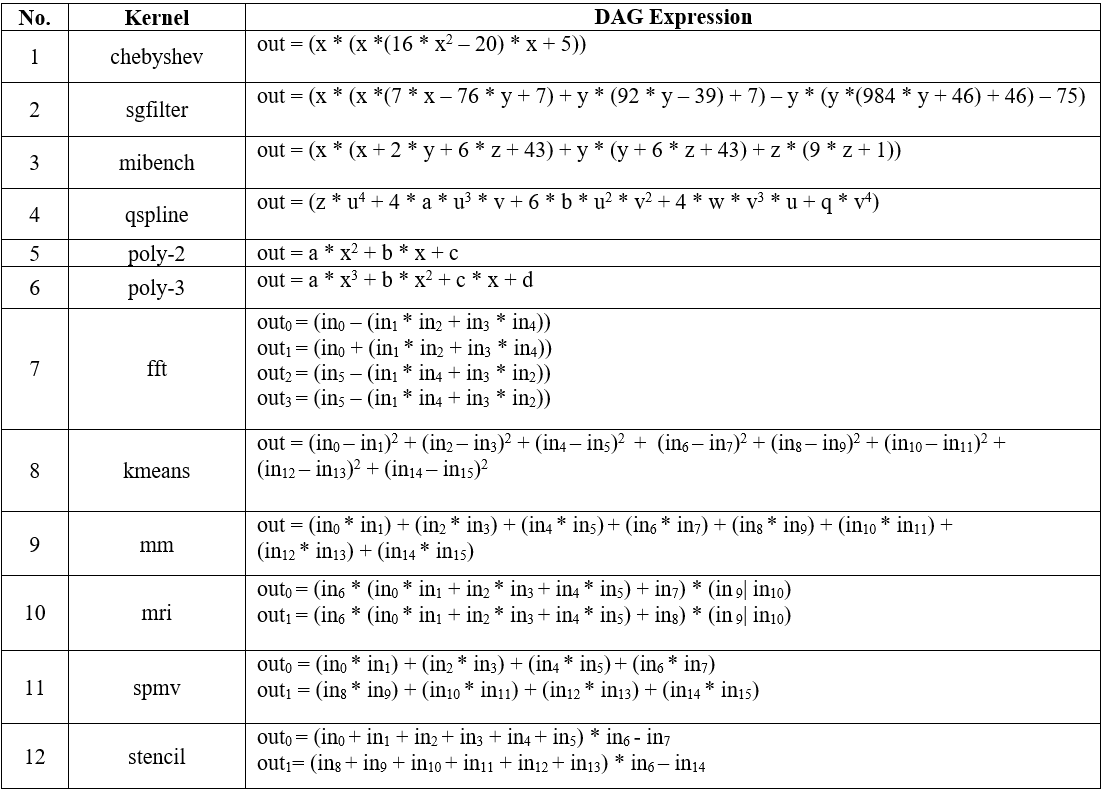
\includegraphics[width=1\textwidth]{images/dag.png}
	\caption{Kernel Benchmarks}
	\label{dag:dag}
\end{table}

\section{Experimentation and Results}

In our work, Xilinx ZedBoard is being used for experimentation and result analysis. We used the gcc for generating the ARM binaries and running the code for the NEON SIMD at the highest optimization level. We used -mfloat-abi=hard -mfpu=neon for running the code on the MXP soft-vector processor.

\subsection{Runtime Comparison}
We compared the runtime for the poly benchmarks (degree-2 and degree-3 polynomial) for huge number of input samples. We observed that MXP outperforms NEON SIMD unit and ARM v7 as it parallelizes the computation and communication. MXP has very high speedups due to the superior double-buffered memory transfer optimization [3.1.3]. The Table~\ref{x:20} and Table~\ref{y:21} represents the runtime in milliseconds for different number of input samples for the poly-2 (quadratic) and poly-3 (cubic) benchmarks respectively. We also plotted a graph between Time in Milliseconds Vs Datasize which shows that the time taken by the MXP soft-vector processor for processing the input samples is very less and provides high speedups. Figure~\ref{dag:q} and Figure~\ref{dag:c} shows the observed runtime for the poly (degree-2 and degree-3) benchmarks. This clearly infers that the MXP soft-vector processor takes less runtime as compared to ARM v7 and Neon while we keep on increasing the number of the input samples. MXP has very high speedups due to the superior double-buffered memory transfer optimization [3.1.3].

\begin{table}[htbp]
	\centering
		\begin{adjustbox}{width=.9\textwidth}
		\small
	\begin{tabular}{lllll}
		\toprule
		\textbf{No of Samples} & \textbf{MXP (ms)} & \textbf{ARMv7 CPU (ms)} & \textbf{INTEL i3 (ms)} & \textbf{NEON(auto vector) (ms)} \\
		\midrule
		$2^{17}$ & 0.4239 & 10 & 0.127 & 0 \\
		$2^{18}$ & 0.884 & 10 & 0.262 & 0 \\
		$2^{19}$ & 1.88 & 10 & 0.654 & 10 \\
		$2^{20}$ & 3.465 & 20 & 1.057 & 10 \\
		$2^{21}$ & 6.949 & 40 & 4.951 & 10 \\
		$2^{22}$ & 13.86 & 70 & 7.962 & 20 \\
		$2^{23}$ & 27.72 & 130 & 9.447 & 40 \\
		$2^{24}$ & 55.46 & 250 & 17.275 & 80 \\
		\bottomrule
	\end{tabular}%
    \end{adjustbox}%
   \caption{Poly-2 Benchmark Runtime in $ms$ for 8-bit data}
	\label{x:20}%
\end{table}%

\begin{table}[htbp]
	\centering
	\begin{adjustbox}{width=.9\textwidth}
		\small
	\begin{tabular}{lllll}
		\toprule
		\textbf{No of Samples} & \textbf{MXP (ms)} & \textbf{ARMv7 CPU (ms)} & \textbf{INTEL i3 (ms)} & \textbf{NEON(auto vector) (ms)} \\
		\midrule
		$2^{17}$ & 0.534 & 10 & 0.127 & 0 \\
		$2^{18}$ & 1.032 & 10 & 0.262 & 0 \\
		$2^{19}$ & 2.064 & 10 & 0.654 & 10 \\
		$2^{20}$ & 4.166 & 30 & 1.057 & 10 \\
		$2^{21}$ & 8.294 & 40 & 4.951 & 20 \\
		$2^{22}$ & 16.50 & 80 & 7.962 & 40 \\
		$2^{23}$ & 33.01 & 160 & 9.447 & 50 \\
		$2^{24}$ & 65.97 & 330 & 17.275 & 80 \\
		
		\bottomrule
	\end{tabular}%
     \end{adjustbox}%
      \caption{Poly-3 Benchmark Runtime in $ms$ for 8-bit data}
	\label{y:21}%
\end{table}%



%% \hfill
%	 \begin{figure}[!b]
%	 \centering 
%	 \begin{tikzpicture}[scale = 1.1]
%	 \begin{semilogyaxis}[
%		xlabel=Datasize$(N)$,
%		ylabel=Time $(ms)$,
%	 % 	scaled ticks=base 10:-5,
%	 xtick pos=left,
%	 ytick pos=left,
%	 ymax = 600,
%	 xmax = 16777216,
%	 yticklabels={1,10,100,1000},
%	 %	symbolic y coords={0.4239,0.847,1.67,3.33,6.69,13.33,26.63,54.41,70,150,290,560},
%	 %  symbolic y coords = {-1,-0.698,-0.522,-0.397,-0.301,-0.221,-0.154,-0.0969,-0.0457,0.0,0.3010,0.4771,0.6021,0.6990,0.7782,0.8450,0.9030,0.9542,1.0,1.3010,1.4771,1.6021,1.6990,1.7782,1.8450,1.9030,1.9542,2.0,2.3010,2.4771,2.6021,2.6990,2.7782,2.8452,2.9030,2.9542,3.0},
%	 %    ytick=data, 
%	 %    yticklabels={0.1,0.2,0.3,0.4,0.5,0.6,0.7,0.8,0.9,1,2,3,4,5,6,7,8,9,10,20,30,40,50,60,70,80,90,100,200,300,400,500,600,700,800,900,1000},
%	 symbolic x coords={131072,262144,524288,1048576,2097152,4194304,8388608,16777216},
%	 enlargelimits=true,
%	 xtick=data,
%	 xticklabels={$2^{17}$,$2^{18}$,$2^{19}$,$2^{20}$,$2^{21}$,$2^{22}$,$2^{23}$,$2^{24}$},
%	 width = 10cm,
%	 xmode = normal,
%	 legend pos=north west,
%	 legend style={draw=none}
%	 ] 
	 
	 
	 % \hfill
	 \begin{figure}[!b]
	 \centering 
	 \begin{tikzpicture}[scale = .8]
	 \begin{semilogyaxis}[
    xlabel=Datasize$(N)$,
	ylabel=Time $(ms)$,
	 % 	scaled ticks=base 10:-5,
	 xtick pos=left,
	 ytick pos=left,
	 ymax = 1000,
	 xmax = 16777216,
	 %	 ymode=log,log ticks with fixed point,
	 %	grid=major,
	 %   symbolic y coords={0.4239, 0.847, 1.67, 3.33, 6.69, 13.33,26.63,54.41},
	 %   ytick={data},
	 symbolic x coords={131072,262144,524288,1048576,2097152,4194304,8388608,16777216},
	 xtick=data,
	 xticklabels={$2^{17}$,$2^{18}$,$2^{19}$,$2^{20}$,$2^{21}$,$2^{22}$,$2^{23}$,$2^{24}$},
	 %	symbolic y coords={0.4239,0.847,1.67,3.33,6.69,13.33,26.63,54.41,70,150,290,560},
	 width = 10cm,
	 xmode = normal,
	 legend pos=north west,
	 legend style={draw=none}
	 ]    
   
	\addplot plot coordinates {
	    (131072,     0.4239)
		(262144,     0.884)
		(524288,    1.88)
		(1048576,    3.465)
		(2097152,    6.949)
		(4194304,    13.86)
		(8388608,   27.72)
		(16777216,   55.46)
		};

%	\addplot plot coordinates {
%	(131072,     0.628)
%	(262144,     1.432)
%	(524288,    2.71)
%	(1048576,    5.266)
%	(2097152,   10.695)
%	(4194304,   21.55)
%	(8388608,   43.143)
%	(16777216,   95.41)
%	
%	};      
	\addplot plot coordinates {
	(131072,     10)
	(262144,     10)
	(524288,    10)
	(1048576,    20)
	(2097152,    40)
	(4194304,    70)
	(8388608,   130)
	(16777216,   250)
	
	};   
   
   	\addplot plot coordinates {
    	(131072,     0)
    	(262144,     0)
    	(524288,    10)
    	(1048576,    10)
    	(2097152,    10)
    	(4194304,    20)
    	(8388608,   40)
    	(16777216,   80)
    
    };   

%	\legend{MXP(Byte)\\Intel i3(Byte)\\ARMv7(Byte)\\Neon(Byte)\\} 
    \legend{MXP(Byte)\\ARMv7(Byte)\\Neon(Byte)\\} 
	\end{semilogyaxis}
	\end{tikzpicture} 
	\label{throughput} 
 \hspace{2.0cm}       $f(samples,time) = a * x ^ 2 + b* x + c$
\caption{Comparing Runtime for \textit{Poly-2} benchmark.} 
\label{dag:q}

\end{figure}

	 % \hfill
	 \begin{figure}[!b]
	 	\centering 
	 	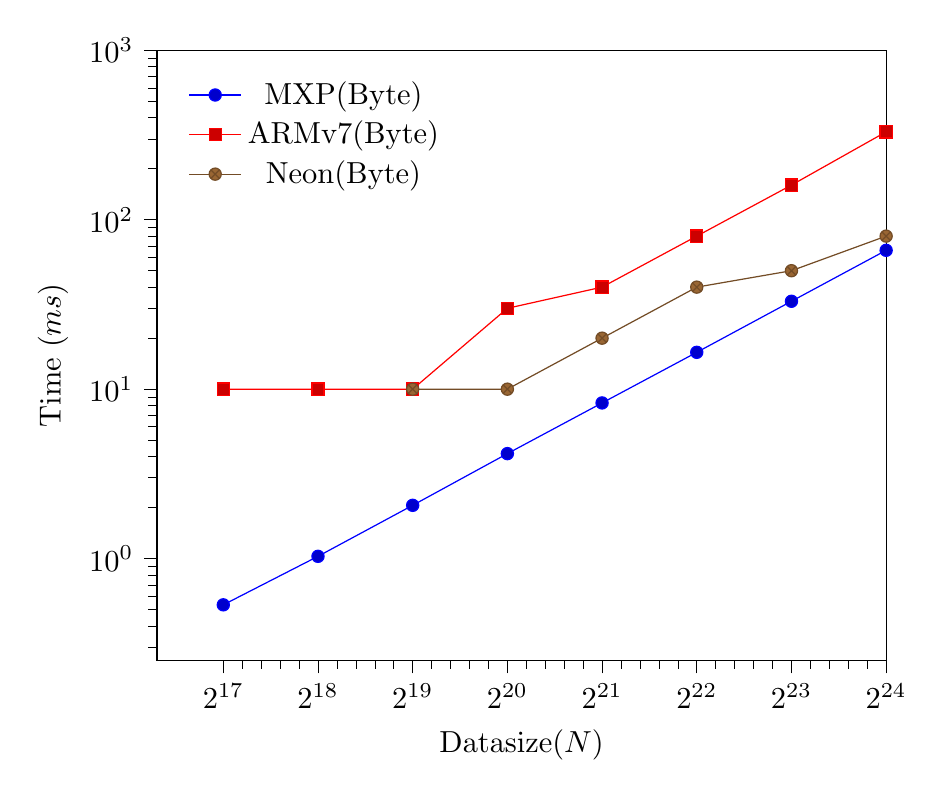
\begin{tikzpicture}[scale = 1.1]
	 	\begin{semilogyaxis}[
	 	xlabel=Datasize$(N)$,
	 	ylabel=Time $(ms)$,
	 	% 	scaled ticks=base 10:-5,
	 	xtick pos=left,
	 	ytick pos=left,
	 	ymax = 1000,
	 	xmax = 16777216,
	 	%	 ymode=log,log ticks with fixed point,
	 	%	grid=major,
	 	%   symbolic y coords={0.4239, 0.847, 1.67, 3.33, 6.69, 13.33,26.63,54.41},
	 	%   ytick={data},
	 	symbolic x coords={131072,262144,524288,1048576,2097152,4194304,8388608,16777216},
	 	xtick=data,
	 	xticklabels={$2^{17}$,$2^{18}$,$2^{19}$,$2^{20}$,$2^{21}$,$2^{22}$,$2^{23}$,$2^{24}$},
	 	%	symbolic y coords={0.4239,0.847,1.67,3.33,6.69,13.33,26.63,54.41,70,150,290,560},
	 	width = 10cm,
	 	xmode = normal,
	 	legend pos=north west,
	 	legend style={draw=none}
	 	]    
	 	
	   	\addplot plot coordinates {
	   		(131072,     0.534)
	   		(262144,     1.032)
	   		(524288,    2.064)
	   		(1048576,    4.166)
	   		(2097152,    8.294)
	   		(4194304,    16.50)
	   		(8388608,   33.01)
	   		(16777216,  65.97)
	   		
	   	};
%	   	\addplot plot coordinates {
%	   		(131072,     0.71)
%	   		(262144,     3.389)
%	   		(524288,    5.86)
%	   		(1048576,    8.431)
%	   		(2097152,   12.075)
%	   		(4194304,   23.431)
%	   		(8388608,   44.572)
%	   		(16777216,   113.9)
%	   		
%	   	};      
	   	\addplot plot coordinates {
	   		(131072,     10)
	   		(262144,     10)
	   		(524288,    10)
	   		(1048576,    30)
	   		(2097152,    40)
	   		(4194304,    80)
	   		(8388608,   160)
	   		(16777216,  330)
	   		
	   	};   
	   	
	   	\addplot plot coordinates {
	   		(131072,     0)
	   		(262144,     0)
	   		(524288,    10)
	   		(1048576,    10)
	   		(2097152,    20)
	   		(4194304,    40)
	   		(8388608,   50)
	   		(16777216,   80)
	   	};   
	   	
	 
%	 \legend{MXP(Byte)\\Intel i3(Byte)\\ARMv7(Byte)\\Neon(Byte)\\} 
	 \legend{MXP(Byte)\\ARMv7(Byte)\\Neon(Byte)\\} 
	 \end{semilogyaxis}
	 \end{tikzpicture} 
	 \label{throughput} 
	}
\hspace{3.5cm}     $f(samples,time) = a * x ^ 3 + b* x ^ 2 + c *x + d$
\caption{Comparing Runtime for \textit{Poly-3} benchmark.} 
\label{dag:c}
	
\end{figure}

\pgfplotsset{
	axis background/.style={fill=none},
	tick style=black,
	tick label style=black,
	grid=both,
	xtick pos=left,
	ytick pos=left,
	tick style={
		major grid style={style=white,line width=1pt},minor grid style=white,
		tick align=outside,
	},
	minor tick num=4,
}

\begin{figure*}[!t]
\centering
\pgfplotstableread{
	0  0.33		0.93	1.5		2.85   
	1  0.4      1.8     2.28	4.74
	2  0.28     0.5     0.75	1.9 
	3  0.35    	0.9     1.14    3.43
	4  0.16    	0.25    0.38    1.77
	5  0.28    	0.43    0.57    2.35
}\dataset
\begin{tikzpicture}
\centering
\begin{axis}[ybar=0pt,
%enlarge x limits=0.05,
width=25cm,
x = 1.8cm,
height=8cm,
ymin=0,
ymax=8,        
ylabel={Throughput in GOPS},
grid style={dotted,gray},
ymajorgrids=true,
nodes near coords,    
xtick=data,
bar width = 0.15,
xticklabels = {
	\strut quad-byte,
	\strut cubic-byte,
	\strut quad-half,
	\strut cubic-half,
	\strut quad-word,
	\strut cubic-word,	                                  
},
x tick label style={rotate=45, anchor=north east, inner sep=0mm},
major x tick style = {opacity=0},
minor x tick num = 1,
minor tick length=1ex,
every node near coord/.append style={
        anchor=west,
        rotate=90,
        font=\tiny
},
]
\addplot[draw=black,fill=blue!90, draw opacity=1] table[x index=0,y index=1] \dataset;\label{ARM} %ano de 2013-2014
\addplot[draw=black,fill=green!90, draw opacity=1] table[x index=0,y index=2] \dataset;\label{NEON} %ano de 2012-2013
\addplot[draw=black,fill=red!90, draw opacity=1] table[x index=0,y index=3] \dataset;\label{MXP} %ano de 2012-2013
\addplot[draw=black,fill=black!90, draw opacity=1] table[x index=0,y index=4] \dataset;\label{Intel-i3} %ano de 2012-2013
\end{axis}
	\node [draw,fill=white] at (rel axis cs: 0.55,0.8) {\shortstack[l]{
			\ref{ARM} ARM \ref{NEON} NEON \ref{MXP} MXP \ref{Intel-i3} Intel-i3}};

\end{tikzpicture}
\caption{The performance comparisons of different architectures for quad and cubic}
\label{throughput}

\end{figure*}



\subsection{Benchmarks Performance Analysis}
In this section, we are going to compare the MXP soft-vector processor with other embedded hard processor such as ARM v7, NEON SIMD unit and INTEL i3. The main criterion of the comparison would be the throughput expressed in terms of Gops/sec.

\subsubsection{Throughput Analysis for poly benchmark}

The compute kernels for the first part of performance comparison work which we took were polynomial with degree-2 (quadratic) and degree-3 (cubic).
We observed that for these benchmarks, MXP has very high throughput when it is operating at the byte(8-bits) level. MXP has very high speedups due to the superior double-buffered memory transfer optimization [3.1.3]. Architecture specification and the corresponding performance in terms of throughput for the poly (degree-2 and degree-3) benchmarks are mentioned in table~\ref{poly:c}.  Figure~\ref{poly:1}, ~\ref{poly:2} and ~\ref{poly:3} demonstrates the average throughput (Gops/sec) obtained while operating on the byte, halfword and word level.

\begin{table}[htbp]
	\centering
	\begin{adjustbox}{width=1\textwidth}
		\small
		\begin{tabular}{llllll}
			\toprule
			\textbf{Metrics} &   & \textbf{ARMv7 CPU} & \textbf{NEON (auto vector)} & \textbf{MXP} & \textbf{INTEL i3} \\
			\midrule
			\textbf{arch} &   & Scalar & SIMD unit & Vector & Scalar \\
			\textbf{clock} &   & $667 X 10^{6}Hz$ & $667 X 10^{6}Hz$ & $110 X 10^{6}Hz$ & $2 X 10^{9}Hz$ \\
			\textbf{no of lanes} &   & 1 & 2 x 32b & 1-16 x 32b & 1 \\
			&   &   & 4 x 16b & 2-32 x 16b &  \\
			&   &   & 8 x 8b & 4-64 x 8b &  \\
			\midrule
			 \textbf{Throughput} & \textbf{Benchmark} &   &   &   &  \\
			\midrule
			 32b(Gops/sec)/ Word   & Quadratic- Poly Deg 2  & 0.1608  & 0.2500 & 0.3782 & 1.77 \\
			 16b(Gops/sec)/Halfword &   & 0.2819 & 0.4988 & 0.758 & 1.914\\
			 8b(Gops/sec)/Byte &   & 0.33656 & 0.9341 & 1.513 & 2.85 \\
			   &   &   &   &   &  \\
			\midrule
			 \textbf{Throughput} & \textbf{Benchmark} &   &   &   &  \\
			\midrule
			 32b(Gops/sec)/ Word   & Cubic- Poly Deg 3    & 0.2886 & 0.4311 & 0.571 & 2.35 \\
			 16b(Gops/sec)/Halfword &   & 0.356 & 0.893 & 1.144 & 3.43 \\
			 8b(Gops/sec)/Byte &   & 0.40054 & 1.7816 & 2.287 & 4.74 \\
			   &   &   &   &   &  \\
			\bottomrule
		\end{tabular}%
	\end{adjustbox}%
	\caption{Throughput(Gops/sec) Analysis for Poly Benchmarks}
	\label{poly:c}%
\end{table}%

%\begin{figure}
%	\centering
%	\begin{tikzpicture}
%	\begin{axis}[
% 	width  = 0.85*\textwidth,
%	height = 8cm,
%	major x tick style = transparent,
%	bar width=10pt,
%	ymajorgrids = true,
%	ylabel = {Throughput in $Gops/sec$},
%	xlabel = {Poly Benchmarks},
%	symbolic x coords={Quadratic Poly-2,Cubic Poly-3},
%	xtick = data,
%	nodes near coords,
%	ybar,
%	every node near coord/.append style={rotate=90, anchor=west, font=\scriptsize,xshift=0.5cm},
%	scaled y ticks = false,
%	enlarge y limits={upper,value=0.2},
%	enlarge x limits=0.25,
%	ybar=2*\pgflinewidth,
%	legend cell align=left,
%	legend style={
%	at={(.5,-0.2)},
%	anchor=north,
%	legend columns=-1
%	column sep=0.5ex
%}
%	]
%	\addplot[draw=black,fill=blue]
%	coordinates {(Quadratic Poly-2, 1.5130) (Cubic Poly-3,2.287)};
%	
%	\addplot[draw=black,fill=orange,every node near coord/.append style={xshift=-0.25cm}]
%	coordinates {(Quadratic Poly-2,2.85) (Cubic Poly-3,4.74)};
%	
%	\addplot[draw=black,fill=yellow,every node near coord/.append style={xshift=-0.70cm}]
%	coordinates {(Quadratic Poly-2,0.336) (Cubic Poly-3,0.40)};
%	
%	\addplot[draw=black,fill=red,every node near coord/.append style={xshift=-1.10cm}]
%	coordinates {(Quadratic Poly-2,0.9341) (Cubic Poly-3,1.732)};
%	
%	\legend{MXP,Intel i3,ARM v7,NEON}
%	\end{axis}
%	\end{tikzpicture}
%	\caption{Byte(8-bits) level throughput(Gops/sec) for polynomial benchmarks }
%	\label{poly:1}
%\end{figure}
\begin{figure}
	\centering
	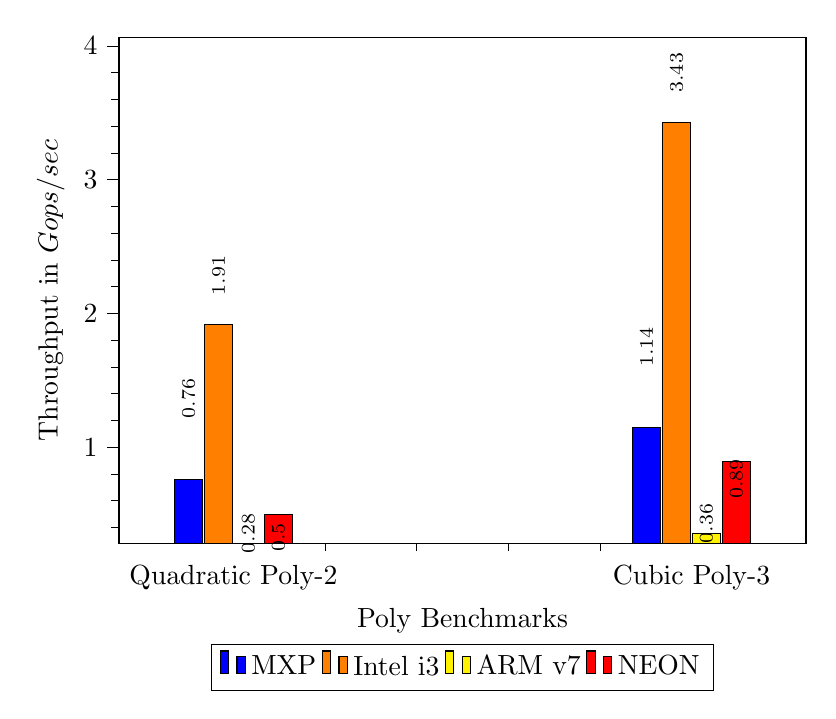
\begin{tikzpicture}
	\begin{axis}[
	width  = 0.85*\textwidth,
	height = 8cm,
	major x tick style = transparent,
	bar width=10pt,
	ymajorgrids = true,
	ylabel = {Throughput in $Gops/sec$},
	xlabel = {Poly Benchmarks},
	symbolic x coords={Quadratic Poly-2,Cubic Poly-3},
	xtick = data,
	nodes near coords,
	ybar,
	every node near coord/.append style={rotate=90, anchor=west, font=\scriptsize, xshift=0.25cm},
	scaled y ticks = false,
	enlarge y limits={upper,value=0.2},
	enlarge x limits=0.25,
	ybar=2*\pgflinewidth,
	legend cell align=left,
		legend style={
		at={(.5,-0.2)},
		anchor=north,
		legend columns=-1
		column sep=0.5ex
	}
	]
	\addplot[draw=black,fill=blue, every node near coord/.append style={xshift=0.4cm}]
	coordinates {(Quadratic Poly-2,0.758 ) (Cubic Poly-3,1.144)};
	
	\addplot[draw=black,fill=orange]
	coordinates {(Quadratic Poly-2,1.914) (Cubic Poly-3,3.43)};
	
	\addplot[draw=black,fill=yellow,every node near coord/.append style={xshift=-0.50cm}]
	coordinates {(Quadratic Poly-2,0.2819) (Cubic Poly-3,0.356)};
	
	\addplot[draw=black,fill=red, every node near coord/.append style={xshift=-0.85cm}]
	coordinates {(Quadratic Poly-2,0.4988) (Cubic Poly-3,0.8939)};
	
	\legend{MXP,Intel i3,ARM v7,NEON}
	\end{axis}
	\end{tikzpicture}
	\caption{Halfword(16-bits) level throughput(Gops/sec) for polynomial benchmarks }
	\label{poly:2}
\end{figure}

\begin{figure}
	\centering
	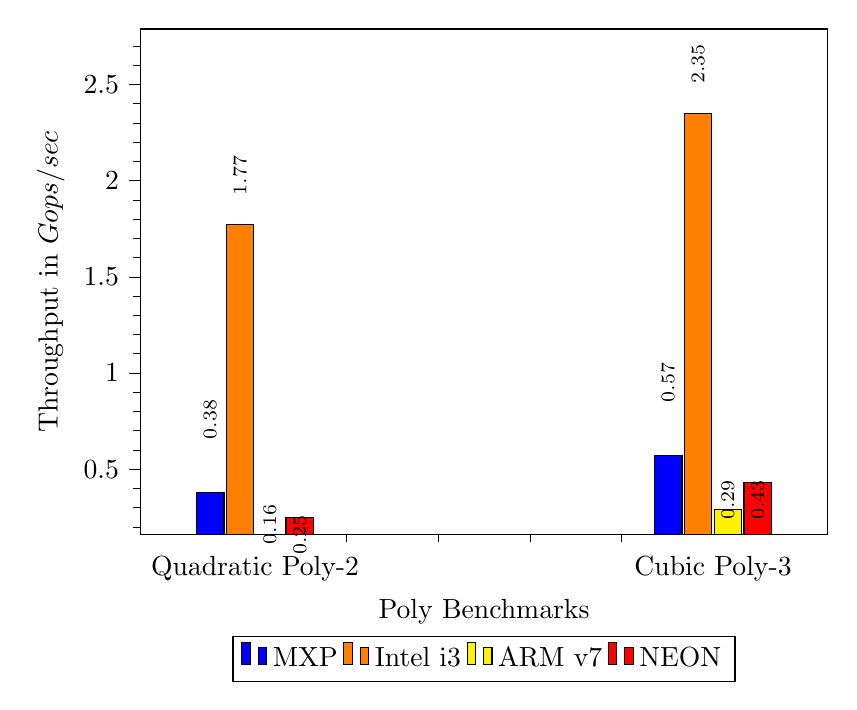
\begin{tikzpicture}
	\begin{axis}[
	width  = 0.85*\textwidth,
	height = 8cm,
	major x tick style = transparent,
	bar width=10pt,
	ymajorgrids = true,
	ylabel = {Throughput in $Gops/sec$},
	xlabel = {Poly Benchmarks},
	symbolic x coords={Quadratic Poly-2,Cubic Poly-3},
	xtick = data,
	nodes near coords,
	ybar,
	every node near coord/.append style={rotate=90, anchor=west,font=\scriptsize, xshift=0.25cm},
	scaled y ticks = false,
	enlarge y limits={upper,value=0.2},
	enlarge x limits=0.25,
	ybar=2*\pgflinewidth,
	legend cell align=left,
		legend style={
		at={(.5,-0.2)},
		anchor=north,
		legend columns=-1
		column sep=0.5ex
	}
	]
	\addplot[draw=black,fill=blue,every node near coord/.append style={xshift=0.3cm}]
	coordinates {(Quadratic Poly-2, 0.378) (Cubic Poly-3,0.571)};
	
	\addplot[draw=black,fill=orange]
	coordinates {(Quadratic Poly-2,1.77) (Cubic Poly-3,2.35)};
	
	\addplot[draw=black,fill=yellow,every node near coord/.append style={xshift=-0.50cm}]
	coordinates {(Quadratic Poly-2,0.1608) (Cubic Poly-3,0.2886)};
	
	\addplot[draw=black,fill=red,every node near coord/.append style={xshift=-0.85cm}]
	coordinates {(Quadratic Poly-2,0.2500) (Cubic Poly-3,0.4311)};
	
	\legend{MXP,Intel i3,ARM v7,NEON}
	\end{axis}
	\end{tikzpicture}
	\caption{Word(32-bits) level throughput(Gops/sec) for polynomial benchmarks }
	\label{poly:3}
\end{figure}



\subsubsection{Throughput Analysis for filter compute kernel}

The compute kernels for second part of performance comparison which we took were the standard filter kernel. Throughput analysis for filter compute Kernels such as Chebyshev, Mibench, Sgfilter and Qspline were done.
We observed that for these benchmarks, MXP has very high throughput when it is operating at the byte(8-bits) level. MXP has very high speedups due to the superior double-buffered memory transfer optimization [3.1.3]. Table~\ref{poly:d} explains the architecture specification and the corresponding throughput obtained in terms of Gops/sec for various benchmarks. Figure~\ref{filter:1}, ~\ref{filter:2} and ~\ref{filter:3} demonstrates the average throughput (Gops/sec) obtained while operating on the word (32-bits), halfword (16- bits) and byte (8-bits) levels.
 We also observed that for a specific benchmark, the performance at the byte level was 4 times and at the halfword level was 2 times when compared with the performance at the word level for the MXP soft-vector processor. For MXP, we have the width of the data as selectable parameter.

\begin{table}[htbp]
	\centering
		\begin{adjustbox}{width=1\textwidth}
		\small
	\begin{tabular}{llllll}
		\toprule
		\textbf{Metrics} &   & \textbf{ARMv7 CPU} & \textbf{NEON (auto vector)} & \textbf{MXP} & \textbf{INTEL i3} \\
		\midrule
		\textbf{arch} &   & Scalar & SIMD unit & Vector & Scalar \\
		\textbf{clock} &   & $667 x 10^{6}Hz$ & $667 x 10^{6}Hz$ & $110 x 10^{6}Hz$ & $2 x 10^{9}Hz$ \\
		\textbf{no of lanes} &   & 1 & 2 x 32b & 1-16 x 32b & 1 \\
		&   &   & 4 x 16b & 2-32 x 16b &  \\
		&   &   & 8 x 8b & 4-64 x 8b &  \\
		&   &   &   &   &  \\
		\midrule
		 \textbf{Throughput} & \textbf{Benchmark} &   &   &   &  \\
		\midrule
		 32b(Gops/sec)/ Word   & CHEBYSHEV & 0.1832 & 0.296 & 0.354 & 2.040 \\
	 16b(Gops/sec)/Halfword &   & 0.1955 & 0.5159 & 0.7085 & 2.186 \\
		 8b(Gops/sec)/Byte &   & 0.2219 & 0.5585 & 1.41 & 2.324 \\
		   &   &   &   &   &  \\
		   &   &   &   &   &  \\
		\midrule
		 \textbf{Throughput} & \textbf{Benchmark} &   &   &   &  \\
		\midrule
		 32b(Gops/sec)/ Word   & MIBENCH & 0.3478 & 0.426 & 0.386 & 3.816 \\
		 16b(Gops/sec)/Halfword &   & 0.352 & 0.7831 & 0.773 & 6.738 \\
		 8b(Gops/sec)/Byte &   & 0.3659 & 0.460 & 1.547 & 3.338 \\
		  &   &   &   &   &  \\
		   &   &   &   &   &  \\
		\midrule
	 \textbf{Throughput} & \textbf{Benchmark} &   &   &   &  \\
		\midrule
	 32b(Gops/sec)/ Word   & QSPLINE & 0.298 & 0.4641 & 0.442 & 2.372 \\
	16b(Gops/sec)/Halfword &   & 0.493 & 1.169 & 0.88 & 13.38 \\
		 8b(Gops/sec)/Byte &   & 0.561 & 2.341 & 1.76 & 5.935 \\
		\bottomrule
	\end{tabular}%
    \end{adjustbox}%

		\caption{Throughput(Gops/sec) Analysis for Filter Benchmarks}
		\label{poly:d}%
\end{table}%
\begin{figure}
	\centering
	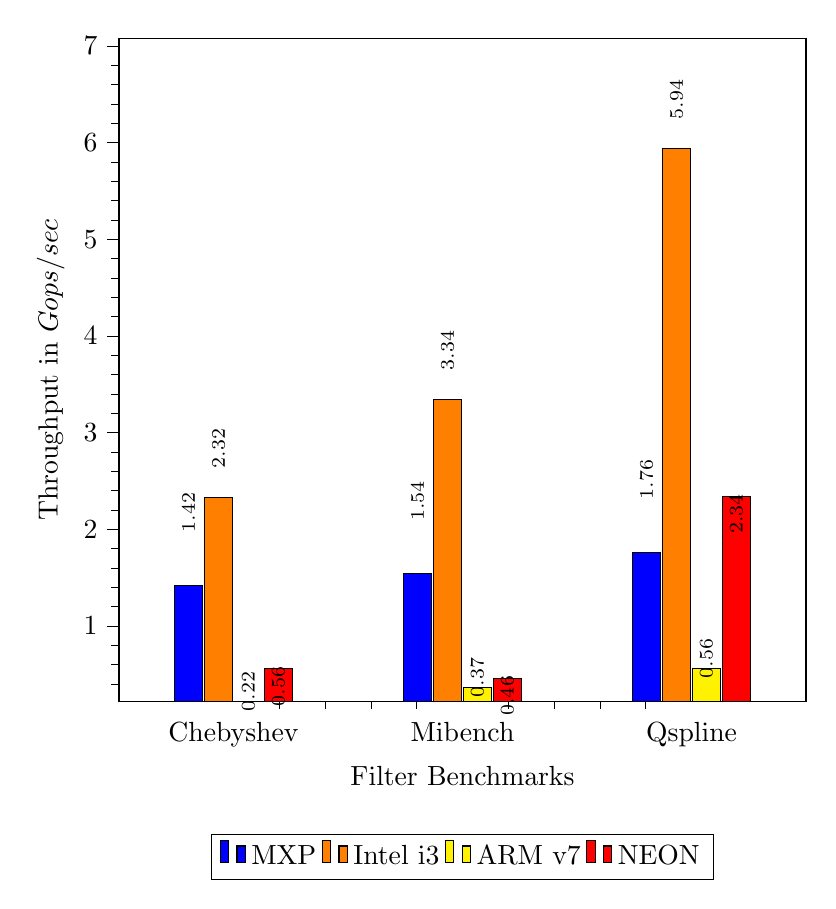
\begin{tikzpicture}
	\begin{axis}[
	width  = 0.85*\textwidth,
	height = 10cm,
	major x tick style = transparent,
	bar width=10pt,
	ymajorgrids = true,
	ylabel = {Throughput in $Gops/sec$},
	xlabel = {Filter Benchmarks},
	symbolic x coords={Chebyshev,Mibench,Qspline},
	xtick = data,
	nodes near coords,
	ybar,
	every node near coord/.append style={rotate=90, anchor=west,font=\scriptsize, xshift=0.25cm},
	scaled y ticks = false,
	enlarge y limits={upper,value=0.2},
	enlarge x limits=0.25,
	ybar=2*\pgflinewidth,
	legend cell align=left,
		legend style={
		at={(.5,-0.2)},
		anchor=north,
		legend columns=-1
		column sep=0.5ex
	}
	]
	\addplot[draw=black,fill=blue, every node near coord/.append style={xshift=.3cm}]
	coordinates {(Chebyshev, 1.417) (Mibench,1.54) (Qspline,1.76)};
	
	\addplot[draw=black,fill=orange]
	coordinates {(Chebyshev, 2.324) (Mibench,3.338) (Qspline,5.935)};
	
	\addplot[draw=black,fill=yellow, every node near coord/.append style={xshift=-0.5cm}]
	coordinates {(Chebyshev, 0.2219) (Mibench,0.3659) (Qspline,0.561)};
	
	\addplot[draw=black,fill=red, every node near coord/.append style={xshift=-0.85cm}]
	coordinates {(Chebyshev, 0.5585) (Mibench,0.460) (Qspline,2.341)};
	
	\legend{MXP,Intel i3,ARM v7,NEON}
	\end{axis}
	\end{tikzpicture}
	\caption{Byte(8-bits) level throughput(Gops/sec) for filter benchmarks }
    \label{filter:1}
\end{figure}

\begin{figure}
	\centering
	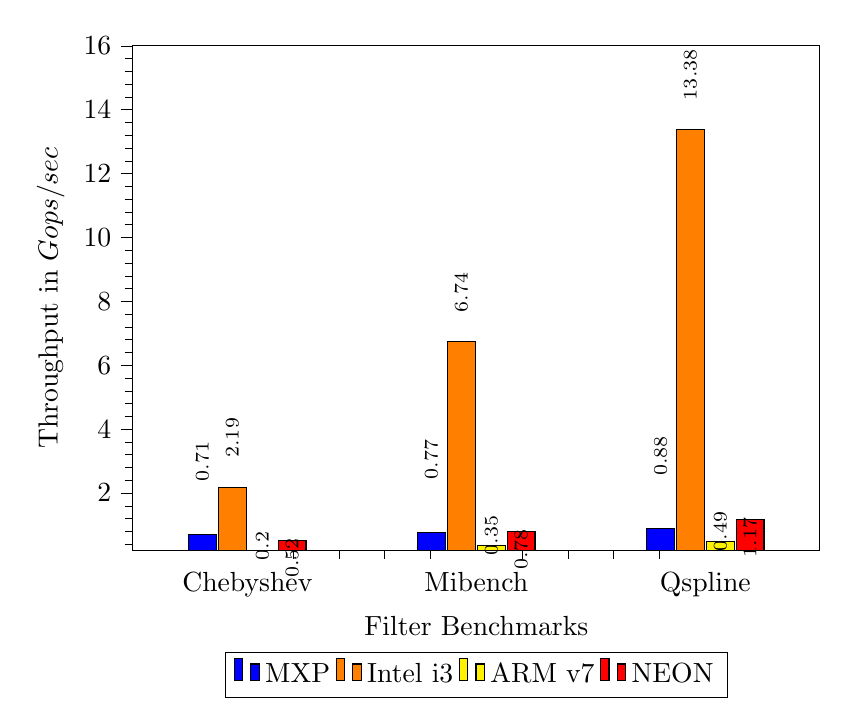
\begin{tikzpicture}
	\begin{axis}[
	width  = 0.85*\textwidth,
	height = 8cm,
	major x tick style = transparent,
	bar width=10pt,
	ymajorgrids = true,
	ylabel = {Throughput in $Gops/sec$},
	xlabel = {Filter Benchmarks},
	symbolic x coords={Chebyshev,Mibench,Qspline},
	xtick = data,
	nodes near coords,
	ybar,
	every node near coord/.append style={rotate=90, anchor=west,font=\scriptsize, xshift=0.25cm},
	scaled y ticks = false,
	enlarge y limits={upper,value=0.2},
	enlarge x limits=0.25,
	ybar=2*\pgflinewidth,
	legend cell align=left,
	legend style={
	at={(.5,-0.2)},
	anchor=north,
	legend columns=-1
	column sep=0.5ex
}
	]
	\addplot[draw=black,fill=blue,every node near coord/.append style={xshift=.3cm}]
	coordinates {(Chebyshev, 0.708) (Mibench,0.77) (Qspline,0.88)};
	
	\addplot[draw=black,fill=orange]
	coordinates {(Chebyshev, 2.186) (Mibench,6.738) (Qspline,13.38)};
	
	\addplot[draw=black,fill=yellow,every node near coord/.append style={xshift=-0.5cm}]
	coordinates {(Chebyshev, 0.1955) (Mibench,0.352) (Qspline,0.493)};
	
	\addplot[draw=black,fill=red,every node near coord/.append style={xshift=-0.85cm}]
	coordinates {(Chebyshev, 0.5159) (Mibench,0.7831) (Qspline,1.169)};
	
	\legend{MXP,Intel i3,ARM v7,NEON}
	\end{axis}
	\end{tikzpicture}
	\caption{Halfword(16-bits) level throughput(Gops/sec) for filter benchmarks }
	\label{filter:2}
\end{figure}
\begin{figure}
	\centering
	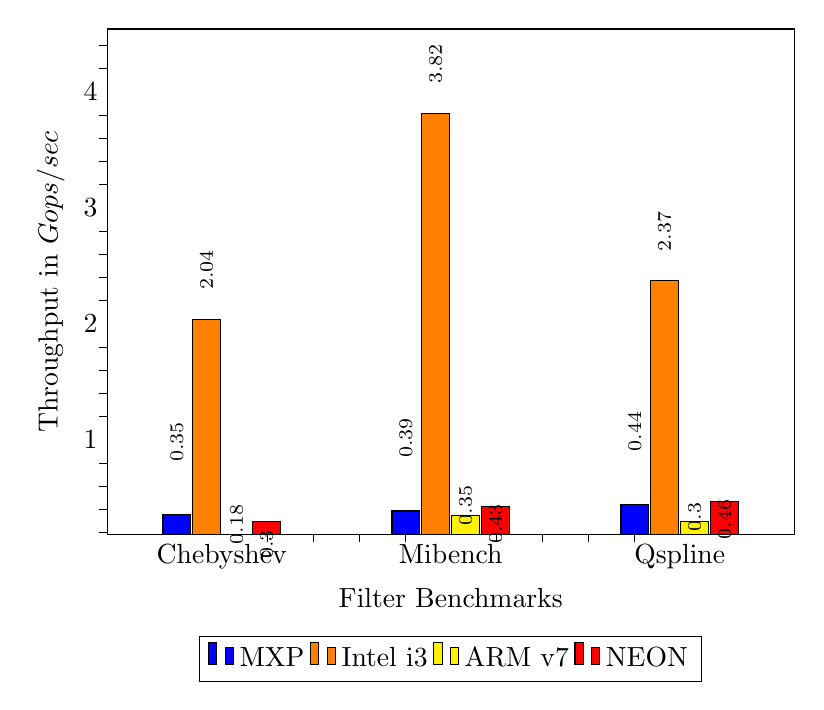
\begin{tikzpicture}
	\begin{axis}[
	width  = 0.85*\textwidth,
	height = 8cm,
	major x tick style = transparent,
	bar width=10pt,
	ymajorgrids = true,
	ylabel = {Throughput in $Gops/sec$},
	xlabel = {Filter Benchmarks},
	symbolic x coords={Chebyshev,Mibench,Qspline},
	major tick length=0cm,
	xtick = data,
	nodes near coords,
	ybar,
	every node near coord/.append style={rotate=90, anchor=west,font=\scriptsize, xshift=0.25cm},
	scaled y ticks = false,
	enlarge y limits={upper,value=0.2},
	enlarge x limits=0.25,
	ybar=2*\pgflinewidth,
	legend cell align=left,
	legend style={
	at={(.5,-0.2)},
	anchor=north,
	legend columns=-1
	column sep=0.5ex
}
	]
	\addplot[draw=black,fill=blue,every node near coord/.append style={xshift=.3cm}]
	coordinates {(Chebyshev, 0.352) (Mibench,0.385) (Qspline,0.44)};
	
	\addplot[draw=black,fill=orange]
	coordinates {(Chebyshev, 2.040) (Mibench,3.816) (Qspline,2.372)};
	
	\addplot[draw=black,fill=yellow, every node near coord/.append style={xshift=-0.5cm}]
	coordinates {(Chebyshev, 0.1832) (Mibench,0.3478) (Qspline,0.298)};
	
	\addplot[draw=black,fill=red, every node near coord/.append style={xshift=-.85cm}]
	coordinates {(Chebyshev, 0.296) (Mibench,0.426) (Qspline,0.4641)};
	
	\legend{MXP,Intel i3,ARM v7,NEON}
	\end{axis}
	\end{tikzpicture}
	\caption{Word(32-bits) level throughput(Gops/sec) for filter benchmarks }
	\label{filter:3}
\end{figure}



\subsubsection{Throughput Analysis for Standard kernels}

As a third part of performance comparison work, we took various benchmarks such as FFT, KMEANS, MM, SPMV, STENCIL and MRI which are the standard compute kernels. We observed that for these compute kernels, MXP has high throughput. MXP has very high speedups due to the superior double-buffered memory transfer optimization [3.1.3]. Table~\ref{poly:a} explains the architecture specification and the corresponding throughput obtained in terms of Gops/sec for various benchmarks. Figure~\ref{kernel:1}, ~\ref{kernel:2}and ~\ref{kernel:3} demonstrates the average throughput (Gops/sec) obtained while operating on the word (32-bits), halfword (16- bits) and byte (8-bits) levels.

\begin{table}[htbp]
	\centering
    	\begin{adjustbox}{width=.8\textwidth}
    	\small
	\begin{tabular}{llllll}
		\toprule
		\textbf{Metrics} &   & \textbf{ARMv7 CPU} & \textbf{NEON (auto vector)} & \textbf{MXP} & \textbf{INTEL i3} \\
		\midrule
		\textbf{arch} &   & Scalar & SIMD unit & Vector & Scalar \\
		\textbf{clock} &   & $667 X 10^{6}Hz$ & $667 X 10^{6}Hz$ & $110 X 10^{6}Hz$ & $2 X 10^{9}Hz$ \\
		\textbf{no of lanes} &   & 1 & 2 x 32b & 1-16 x 32b & 1 \\
		&   &   & 4 x 16b & 2-32 x 16b &  \\
		&   &   & 8 x 8b & 4-64 x 8b &  \\
		\midrule
		  \textbf{Throughput} & \textbf{Benchmark} &   &   &   &  \\
		\midrule
		  32b(Gops/sec)/ Word   & FFT & 0.0867 & 0.137 & 0.174 & 1.0283 \\
		  16b(Gops/sec)/Halfword &   & 0.0937 & 0.2887 & 0.349 & 2.01 \\
		  8b(Gops/sec)/Byte &   & 0.1042 & 0.5833 & 0.6995 & 3.809 \\
		    &   &   &   &   &  \\
		\midrule
		  \textbf{Throughput} & \textbf{Benchmark} &   &   &   &  \\
		\midrule
		  32b(Gops/sec)/ Word   & KMEANS & 0.03174 & 0.09083 & 0.2285 & 1.918 \\
		  16b(Gops/sec)/Halfword &   & 0.06582 & 0.257 & 0.457 & 5.301 \\
		  8b(Gops/sec)/Byte &   & 0.0986 & 0.689 & 0.9143 & 6.96 \\
		    &   &   &   &   &  \\
		\midrule
		  \textbf{Throughput} & \textbf{Benchmark} &   &   &   &  \\
		\midrule
		  32b(Gops/sec)/ Word   & MM & 0.02015 & 0.06009 & 0.156 & 1.24 \\
		  16b(Gops/sec)/Halfword &   & 0.03806 & 0.165 & 0.3136 & 3.456 \\
		  8b(Gops/sec)/Byte &   & 0.0667 & 0.443 & 0.627 & 3.495 \\
		    &   &   &   &   &  \\
		\midrule
		  \textbf{Throughput} & \textbf{Benchmark} &   &   &   &  \\
		\midrule
		  32b(Gops/sec)/ Word   & SPMV & 0.01680 & 0.0532 & 0.1399 & 1.126 \\
		  16b(Gops/sec)/Halfword &   & 0.0307 & 0.1529 & 0.279 & 2.696 \\
		  8b(Gops/sec)/Byte &   & 0.061 & 0.391 & 0.5596 & 3.05 \\
		    &   &   &   &   &  \\
		\midrule
		  \textbf{Throughput} & \textbf{Benchmark} &   &   &   &  \\
		\midrule
		  32b(Gops/sec)/ Word   & STENCIL & 0.03589 & 0.05866 & 0.14 & 1.437 \\
		  16b(Gops/sec)/Halfword &   & 0.0534 & 0.1146 & 0.29 & 2.57 \\
		  8b(Gops/sec)/Byte &   & 0.0651 & 0.1162 & 0.589 & 2.35 \\
		    &   &   &   &   &  \\
		\midrule
		  \textbf{Throughput} & \textbf{Benchmark} &   &   &   &  \\
		\midrule
		  32b(Gops/sec)/ Word   & MRI & 0.039 & 0.077 & 0.097 & 1.221 \\
		  16b(Gops/sec)/Halfword &   & 0.0537 & 0.183 & 0.194 & 2.36 \\
		  8b(Gops/sec)/Byte &   & 0.064 & 0.277 & 0.388 & 1.406 \\
		\bottomrule
	\end{tabular}%
\end{adjustbox}%
	\caption{Throughput(Gops/sec) Analysis for Standard Compute Kernels}
		\label{poly:a}%
\end{table}%

\begin{figure}
	\centering
	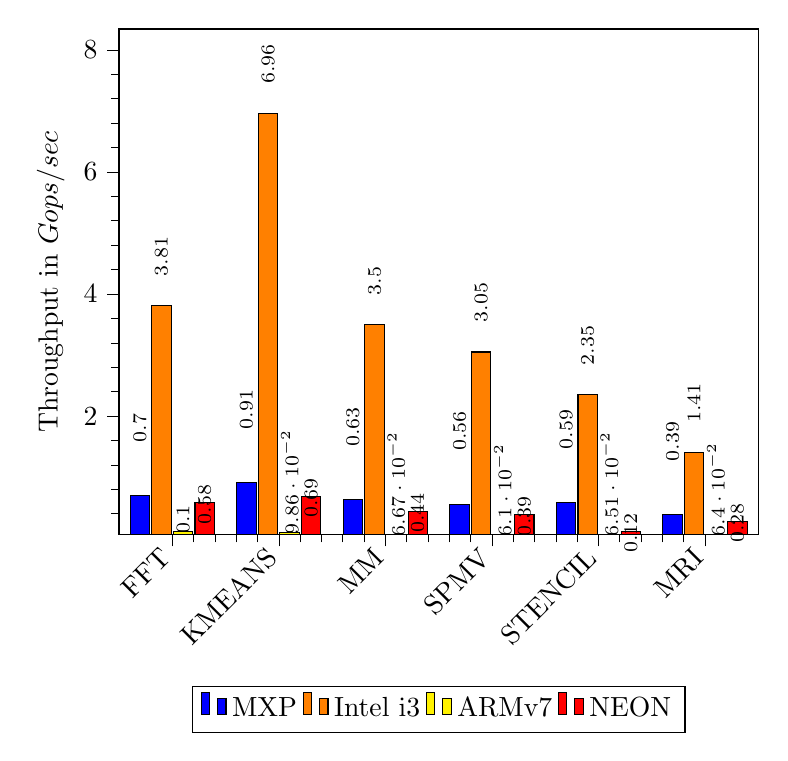
\begin{tikzpicture}
	\begin{axis}[
	width  = 0.8*\textwidth,
	height = 8cm,
	xtick pos=left,
    ytick pos=left,
%	major x tick style = transparent,
	x tick label style={rotate=45, anchor=east, align=right,text width=2cm},
	bar width=7pt,
	ymajorgrids = true,
	ylabel = {Throughput in $Gops/sec$},
	symbolic x coords={FFT,KMEANS,MM,SPMV,STENCIL,MRI},
	xtick = data,
	nodes near coords,
	ybar,
	every node near coord/.append style={rotate=90, anchor=west,font=\scriptsize, xshift=0.25cm},
	scaled y ticks = false,
	enlarge y limits={upper,value=0.2},
%	enlarge x limits=0.25,
	ybar=2*\pgflinewidth,
	legend cell align=left,
	legend style={
	at={(.5,-0.3)},
	anchor=north,
	legend columns=-1
	column sep=0.5ex
}
	]
	\addplot[draw=black,fill=blue,every node near coord/.append style={xshift=0.3cm}]
	coordinates {(FFT, 0.69951) (KMEANS,0.914) (MM,0.627) (SPMV,0.559) (STENCIL,0.589) (MRI,0.388)};
	
	\addplot[draw=black,fill=orange]
	coordinates  {(FFT,3.809) (KMEANS,6.96) (MM,3.495) (SPMV,3.05) (STENCIL,2.35) (MRI,1.406)};
	
	\addplot[draw=black,fill=yellow,every node near coord/.append style={xshift=-0.4cm}]
	coordinates  {(FFT,0.1042) (KMEANS,0.0986) (MM,0.0667) (SPMV,0.061) (STENCIL,0.0651) (MRI,0.064)};
	
	\addplot[draw=black,fill=red,every node near coord/.append style={xshift=-0.65cm}]
	coordinates {(FFT, 0.5833) (KMEANS,0.689) (MM,0.443) (SPMV,0.391) (STENCIL,0.1162) (MRI,0.277)};
	
	\legend{MXP,Intel i3,ARMv7,NEON}
	\end{axis}
	\end{tikzpicture}
	\caption{Byte(8-bits) level throughput(Gops/sec) for compute Kernels}
	\label{kernel:1}
\end{figure}



\begin{figure}
	\centering
	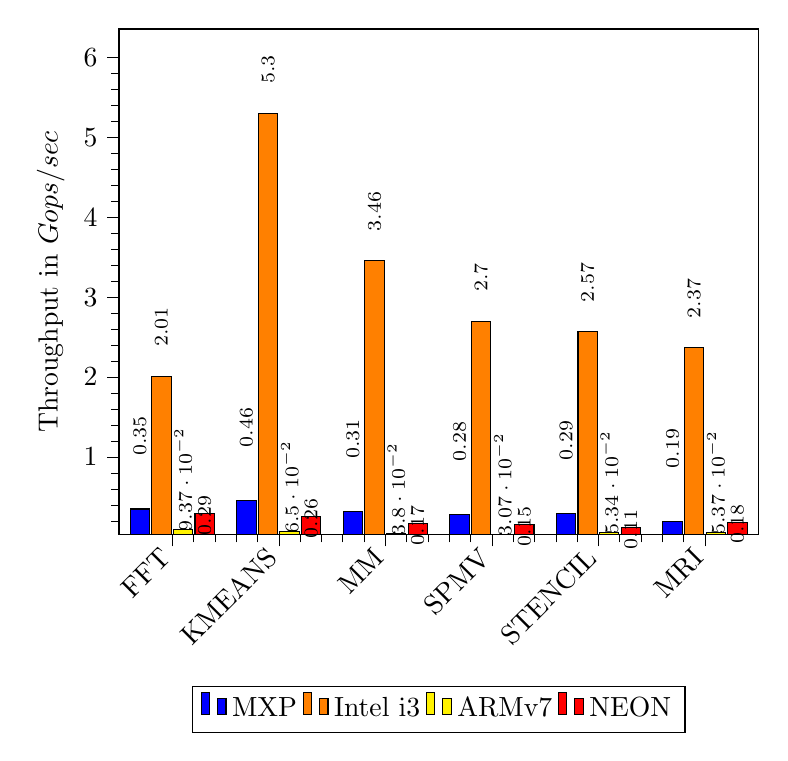
\begin{tikzpicture}
	\begin{axis}[
	width  = 0.8*\textwidth,
	height = 8cm,
	xtick pos=left,
	ytick pos=left,
%	major x tick style = transparent,
	x tick label style={rotate=45, anchor=east, align=right,text width=2cm},
	bar width=7pt,
	ymajorgrids = true,
	ylabel = {Throughput in $Gops/sec$},
	symbolic x coords={FFT,KMEANS,MM,SPMV,STENCIL,MRI},
	xtick = data,
	nodes near coords,
	ybar,
	every node near coord/.append style={rotate=90, anchor=west,font=\scriptsize, xshift=0.25cm},
	scaled y ticks = false,
	enlarge y limits={upper,value=0.2},
%	enlarge x limits=0.25,
	ybar=2*\pgflinewidth,
	legend cell align=left,
	legend style={
		at={(.5,-0.3)},
		anchor=north,
		legend columns=-1
		column sep=0.5ex
	}
	]
	\addplot[draw=black,fill=blue,every node near coord/.append style={xshift=.3cm}]
	coordinates {(FFT, 0.349) (KMEANS,0.457) (MM,0.313) (SPMV,0.2798) (STENCIL,0.294) (MRI,0.194)};
	
	\addplot[draw=black,fill=orange]
	coordinates  {(FFT, 2.01) (KMEANS,5.301) (MM,3.456) (SPMV,2.696) (STENCIL,2.57) (MRI,2.368)};
	
	\addplot[draw=black,fill=yellow,every node near coord/.append style={xshift=-0.4cm}]
	coordinates  {(FFT,0.0937) (KMEANS,0.065) (MM,0.038) (SPMV,0.0307) (STENCIL,0.0534) (MRI,0.0537)};
	
	\addplot[draw=black,fill=red,every node near coord/.append style={xshift=-0.65cm}]
	coordinates {(FFT, 0.2887) (KMEANS,0.257) (MM,0.165) (SPMV,0.1529) (STENCIL,0.1146) (MRI,0.1839)};
	
	\legend{MXP,Intel i3,ARMv7,NEON}
	\end{axis}
	\end{tikzpicture}
	\caption{Halfword(16-bits) level throughput(Gops/sec) for compute Kernels}
	\label{kernel:2}
\end{figure}

\begin{figure}
	\centering
	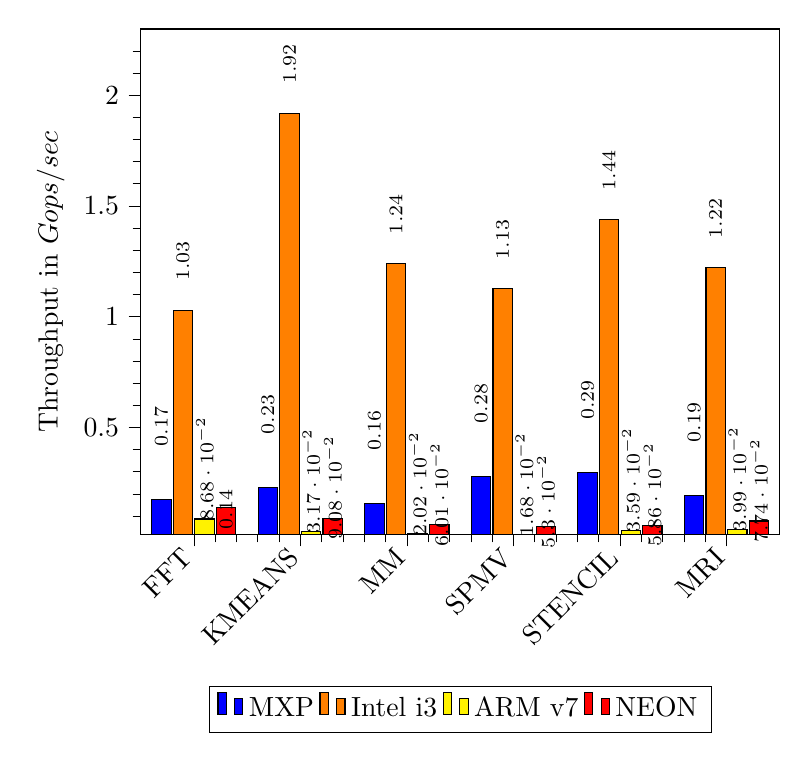
\begin{tikzpicture}
	\begin{axis}[
	width  = 0.8*\textwidth,
	height = 8cm,
	xtick pos=left,
	ytick pos=left,
%	major x tick style = transparent,
	x tick label style={rotate=45, anchor=east, align=right,text width=2cm},
	bar width=7pt,
	ymajorgrids = true,
	ylabel = {Throughput in $Gops/sec$},
	symbolic x coords={FFT,KMEANS,MM,SPMV,STENCIL,MRI},
	xtick = data,
	nodes near coords,
	ybar,
	every node near coord/.append style={rotate=90, anchor=west,font=\scriptsize, xshift=0.25cm},
	scaled y ticks = false,
	enlarge y limits={upper,value=0.2},
%	enlarge x limits=0.25,
	ybar=2*\pgflinewidth,
	legend cell align=left,
	legend style={
	at={(.5,-0.3)},
	anchor=north,
	legend columns=-1
	column sep=0.5ex
}
	]
	\addplot[draw=black,fill=blue,every node near coord/.append style={xshift=0.3cm}]
	coordinates {(FFT,0.174) (KMEANS,0.2285) (MM,0.1567) (SPMV,0.2798) (STENCIL,0.2945) (MRI,0.194)};
	
	\addplot[draw=black,fill=orange]
	coordinates  {(FFT,1.0283) (KMEANS,1.918) (MM,1.24) (SPMV,1.126) (STENCIL,1.437) (MRI,1.2211)};
	
	\addplot[draw=black,fill=yellow,every node near coord/.append style={xshift=-0.4cm}]
	coordinates  {(FFT, 0.08677) (KMEANS,0.03174) (MM,0.02015) (SPMV,0.01680) (STENCIL,0.03589) (MRI,0.0399)};
	
	\addplot[draw=black,fill=red,every node near coord/.append style={xshift=-0.65cm}]
	coordinates {(FFT, 0.13705) (KMEANS,0.0908) (MM,0.06009) (SPMV,0.053) (STENCIL,0.0586) (MRI,0.07735)};
	
	\legend{MXP,Intel i3,ARM v7,NEON}
	\end{axis}
	\end{tikzpicture}
	\caption{Word(32-bits) level throughput(Gops/sec) for compute Kernels}
	\label{kernel:3}
\end{figure}

\subsubsection{Throughput Analysis for Linear Algebra Kernel}

We accelerate two linear algebra kernels namely atax and bicg using MXP overlay. We change the default data type which is double to integer for the computations to have proper comparison analysis about the speedup. We accelerate the kernel for a small dataset with size of matrix 500x500 and for standard dataset size of matrix 4000x4000. The speedup obtained using MXP is as shown in the below table~\ref{lin:a}. We observed that MXP provide high speedup for small as well as standard dataset. For the BiCG kernel, MXP provide speedup of 3 for the small dataset and 3.25 for the standard dataset when compared with the embedded hard processor ARM v7. For ATAX compute kernel, speedup was observed to be 5.62 for the small dataset and 4.63 for standard dataset.



% Table generated by Excel2LaTeX from sheet 'Sheet1'
\begin{table}[htbp]
	\centering
	\begin{adjustbox}{width= .8\textwidth}
		\small
		\begin{tabular}{rrrrr}
			\toprule
			\multicolumn{1}{l}{\textbf{Metrics}} &   & \multicolumn{1}{l}{\textbf{ARMv7 CPU}} & \multicolumn{1}{l}{\textbf{MXP}} & \multicolumn{1}{l}{\textbf{NEON(auto vector)}} \\
			\midrule
			\multicolumn{1}{l}{\textbf{uarch}} &   & \multicolumn{1}{l}{Scalar} & \multicolumn{1}{l}{Soft vector} & \multicolumn{1}{l}{SIMD unit} \\
			\multicolumn{1}{l}{\textbf{Clock}} &   & \multicolumn{1}{l}{667 Mhz} & \multicolumn{1}{l}{110 Mhz} & \multicolumn{1}{l}{667 Mhz} \\
			\multicolumn{1}{l}{\textbf{No of Lanes}} &   & \multicolumn{1}{l}{1} & \multicolumn{1}{l}{1-16 X32b} & \multicolumn{1}{l}{2 X32b} \\
			&   &   & \multicolumn{1}{l}{2-32 X16b} & \multicolumn{1}{l}{4 X16b} \\
			&   &   & \multicolumn{1}{l}{4-64 X8b} & \multicolumn{1}{l}{8 X8b} \\
			\midrule
			\multicolumn{1}{l}{\textbf{Runtime (ms)}} & \multicolumn{1}{l}{\textbf{Benchmark}} &   &   &  \\
			\midrule
			\multicolumn{1}{l}{500 X 500 (small dataset)} & \multicolumn{1}{l}{BiCG} & \multicolumn{1}{l}{5.935} & \multicolumn{1}{l}{1.972} & \multicolumn{1}{l}{5.89} \\
			&   &   &   &  \\
			\multicolumn{1}{l}{4000 X 4000 (standard dataset)} &   & \multicolumn{1}{l}{234.69} & \multicolumn{1}{l}{72.033} & \multicolumn{1}{l}{216.26} \\
			&   &   &   &  \\
			\midrule
			\multicolumn{1}{l}{\textbf{Runtime (ms)}} & \multicolumn{1}{l}{\textbf{Benchmark}} &   &   &  \\
			\midrule
			\multicolumn{1}{l}{500 X 500 (small dataset)} & \multicolumn{1}{l}{ATAX} & \multicolumn{1}{l}{6.598} & \multicolumn{1}{l}{1.172} & \multicolumn{1}{l}{6.581} \\
			&   &   &   &  \\
			\multicolumn{1}{l}{4000 X 4000 (standard dataset)} &   & \multicolumn{1}{l}{486.96} & \multicolumn{1}{l}{105.303} & \multicolumn{1}{l}{483.99} \\
			&   &   &   &  \\
			\bottomrule
		\end{tabular}%
	\end{adjustbox}%
	\caption{Throughput(Gops/sec) Analysis for Linear Algebra kernel}
	\label{lin:a}%	
\end{table}%


    
    
    \subsubsection{Speedup Analysis w.r.t ARM cortex A9}
    Speedup analysis for MXP, SIMD NEON and INTEL i3 was obtained taking ARM Cortex A9 as the reference processor. The DFG processing for the various kernels on MXP is summarized in this section. The speedup factors were calculated for standard kernels at the byte, halfword and the word level. The analysis shows that when we are operating at the byte level the MXP provides the four times parallelism and hence is supposed to give high speedup as compared to other processors. Figure~\ref{speedup:1} demonstrates the byte level speedup obtained with respect to the ARM cortex A9 processor. It can be inferred that the MXP provides high speedup for the kernel with much more computation as MXP make use of the overlapping of communication and computation feature to hide the time incurred in transferring the data. Figure~\ref{speedup:2} and Figure~\ref{speedup:3} demonstrates the halfword and the word level speedup obtained with respect to the ARM cortex A9 processor. With respect to these graphs it can be observed that the INTEL i3 processor have some better speedup for kernels requiring high computation.
  
  
  
\begin{figure}
	\centering
	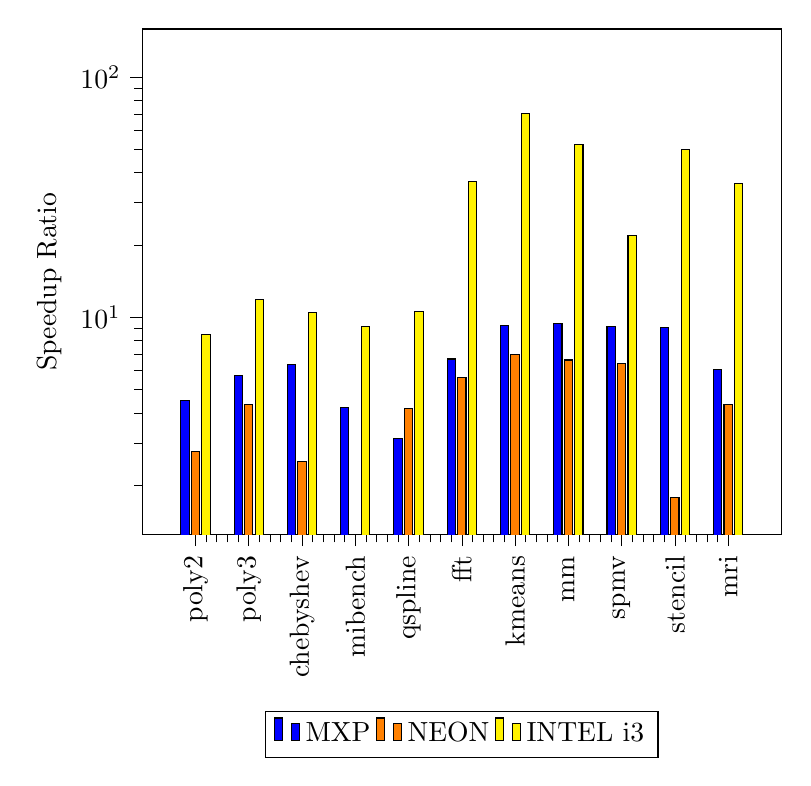
\begin{tikzpicture}
	\begin{semilogyaxis}[
	width  = 0.8*\textwidth,
	height = 8cm,
	xtick pos=left,
	ytick pos=left,
	%	major x tick style = transparent,
	x tick label style={rotate=90, anchor=east, align=right,text width=2cm},
	bar width=3pt,
	ymajorgrids = true,
	ylabel = {Speedup Ratio},
	symbolic x coords={poly2,poly3,chebyshev,mibench,qspline,fft,kmeans,mm,spmv,stencil,mri},
	xtick = data,
%	nodes near coords,
%	ybar,
%	every node near coord/.append style={rotate=90, anchor=west,font=\tiny, xshift=0.25cm},
	%	nodes near coords,
	%	ybar,
	%	every node near coord/.append style={rotate=90, anchor=west,font=\scriptsize},
	scaled y ticks = false,
	enlarge y limits={upper,value=0.2},
	%test
	%	enlarge x limits=0.25,
	ybar=2*\pgflinewidth,
	legend cell align=left,
	legend style={
		at={(.5,-0.35)},
		anchor=north,
		legend columns=-1
		column sep=0.5ex
	}
	]
	\addplot[draw=black,fill=blue]
	coordinates {(poly2,4.49) (poly3,5.709) (chebyshev,6.386) (mibench,4.22) (qspline,3.13) (fft,6.71) (kmeans,9.26) (mm,9.400) (spmv,9.1737) (stencil,9.0538) (mri,6.059) };
	
	\addplot[draw=black,fill=orange]
	coordinates	{(poly2,2.775 ) (poly3,4.32) (chebyshev,2.51) (mibench,1.25) (qspline,4.17) (fft,5.597) (kmeans,6.983) (mm,6.641) (spmv,6.4098) (stencil,1.784) (mri,4.326) };
	
	\addplot[draw=black,fill=yellow]
	coordinates	{(poly2,8.469 ) (poly3,11.834) (chebyshev,10.47) (mibench,9.122) (qspline,10.57) (fft,36.55) (kmeans,70.54) (mm,52.39) (spmv,21.96) (stencil,50) (mri,36.098) };
	
	\legend{MXP,NEON,INTEL i3}
	\end{semilogyaxis}	
	\end{tikzpicture}
	\caption{Byte level Speedup Analysis w.r.t ARMv7 for  different benchmarks.}
	\label{speedup:1}
\end{figure}

   
 
 \begin{figure}
 	\centering
 	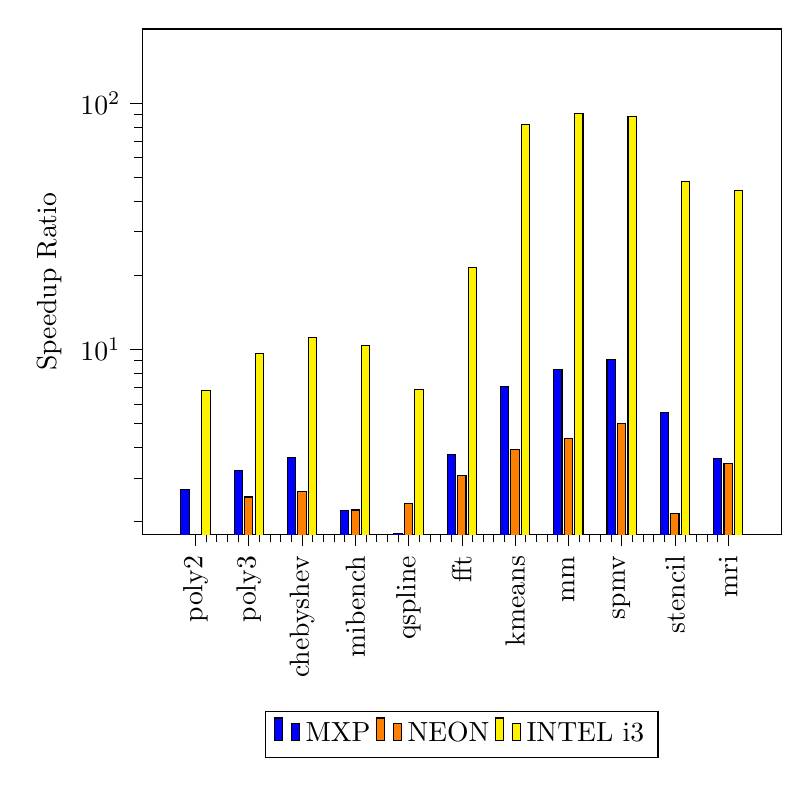
\begin{tikzpicture}
 	\begin{semilogyaxis}[
 	width  = 0.8*\textwidth,
 	height = 8cm,
 	xtick pos=left,
 	ytick pos=left,
 	%	major x tick style = transparent,
 	x tick label style={rotate=90, anchor=east, align=right,text width=2cm},
 	bar width=3pt,
 	ymajorgrids = true,
 	ylabel = {Speedup Ratio},
 	symbolic x coords={poly2,poly3,chebyshev,mibench,qspline,fft,kmeans,mm,spmv,stencil,mri},
 	xtick = data,
% 	nodes near coords,
% 	ybar,
% 	every node near coord/.append style={rotate=90, anchor=west,font=\tiny},
 	scaled y ticks = false,
 	enlarge y limits={upper,value=0.2},
 	%test
 	%	enlarge x limits=0.25,
 	ybar=2*\pgflinewidth,
 	legend cell align=left,
 	legend style={
 		at={(.5,-0.35)},
 		anchor=north,
 		legend columns=-1
 		column sep=0.5ex
 	}
 	]
 	\addplot[draw=black,fill=blue]
 	coordinates {(poly2,2.683) (poly3,3.21) (chebyshev,3.62) (mibench,2.216) (qspline,1.784) (fft,3.729) (kmeans,7.033) (mm,8.25) (spmv,9.11) (stencil,5.51) (mri,3.61) };
 	
 	\addplot[draw=black,fill=orange]
 	coordinates	{(poly2,1.769 ) (poly3,2.51) (chebyshev,2.638) (mibench,2.224) (qspline,2.3711) (fft,3.0811) (kmeans,3.90) (mm,4.335) (spmv,4.980) (stencil,2.146) (mri,3.424) };
 	
 	\addplot[draw=black,fill=yellow]
 	coordinates	{(poly2,6.78 ) (poly3,9.634) (chebyshev,11.18) (mibench,10.38) (qspline,6.855) (fft,21.45) (kmeans,81.5) (mm,90.8) (spmv,87.81) (stencil,48.12) (mri,44) };
 	
 	\legend{MXP,NEON,INTEL i3}
 	\end{semilogyaxis}	
 	\end{tikzpicture}
 	\caption{Half Word level Speedup Analysis w.r.t ARMv7 for  different benchmarks.}
 	\label{speedup:2}
 \end{figure}
 

  

\begin{figure}
	\centering
	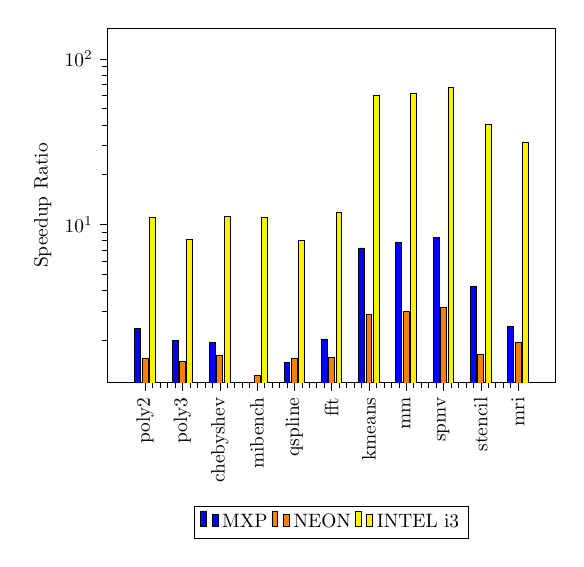
\begin{tikzpicture}[scale=0.7]
	\begin{semilogyaxis}[
	width  = 0.8*\textwidth,
	height = 8cm,
	xtick pos=left,
	ytick pos=left,
	%	major x tick style = transparent,
	x tick label style={rotate=90, anchor=east, align=right,text width=2cm},
	bar width=3pt,
	ymajorgrids = true,
	ylabel = {Speedup Ratio},
	symbolic x coords={poly2,poly3,chebyshev,mibench,qspline,fft,kmeans,mm,spmv,stencil,mri},
	xtick = data,
%	nodes near coords,
%	ybar,
%	every node near coord/.append style={rotate=90, anchor=west,font=\tiny},
	scaled y ticks = false,
	enlarge y limits={upper,value=0.2},
	%test
	%	enlarge x limits=0.25,
	ybar=2*\pgflinewidth,
	legend cell align=left,
	legend style={
		at={(.5,-0.35)},
		anchor=north,
		legend columns=-1
		column sep=0.5ex
	}
	]
	\addplot[draw=black,fill=blue]
	coordinates {(poly2,2.35) (poly3,1.98) (chebyshev,1.933) (mibench,1.11) (qspline,1.47) (fft,2.033) (kmeans,7.20) (mm,7.779) (spmv,8.32) (stencil,4.20) (mri,2.42) };
	
	\addplot[draw=black,fill=orange]
	coordinates	{(poly2,1.55 ) (poly3,1.49) (chebyshev,1.61) (mibench,1.22) (qspline,1.55) (fft,1.58) (kmeans,2.86) (mm,2.98) (spmv,3.16) (stencil,1.63) (mri,1.934) };
	
	\addplot[draw=black,fill=yellow]
	coordinates	{(poly2,11 ) (poly3,8.14) (chebyshev,11.13) (mibench,10.97) (qspline,7.95) (fft,11.85) (kmeans,60.42) (mm,61.53) (spmv,67.023) (stencil,40.039) (mri,31.28) };
	
	\legend{MXP,NEON,INTEL i3}
	\end{semilogyaxis}	
	\end{tikzpicture}
	\caption{Word level Speedup Analysis w.r.t ARMv7 for  different benchmarks.}
	\label{speedup:3}
\end{figure}

  
  
  
 
  
  
  
%    \begin{figure}
%    	\centering
%    	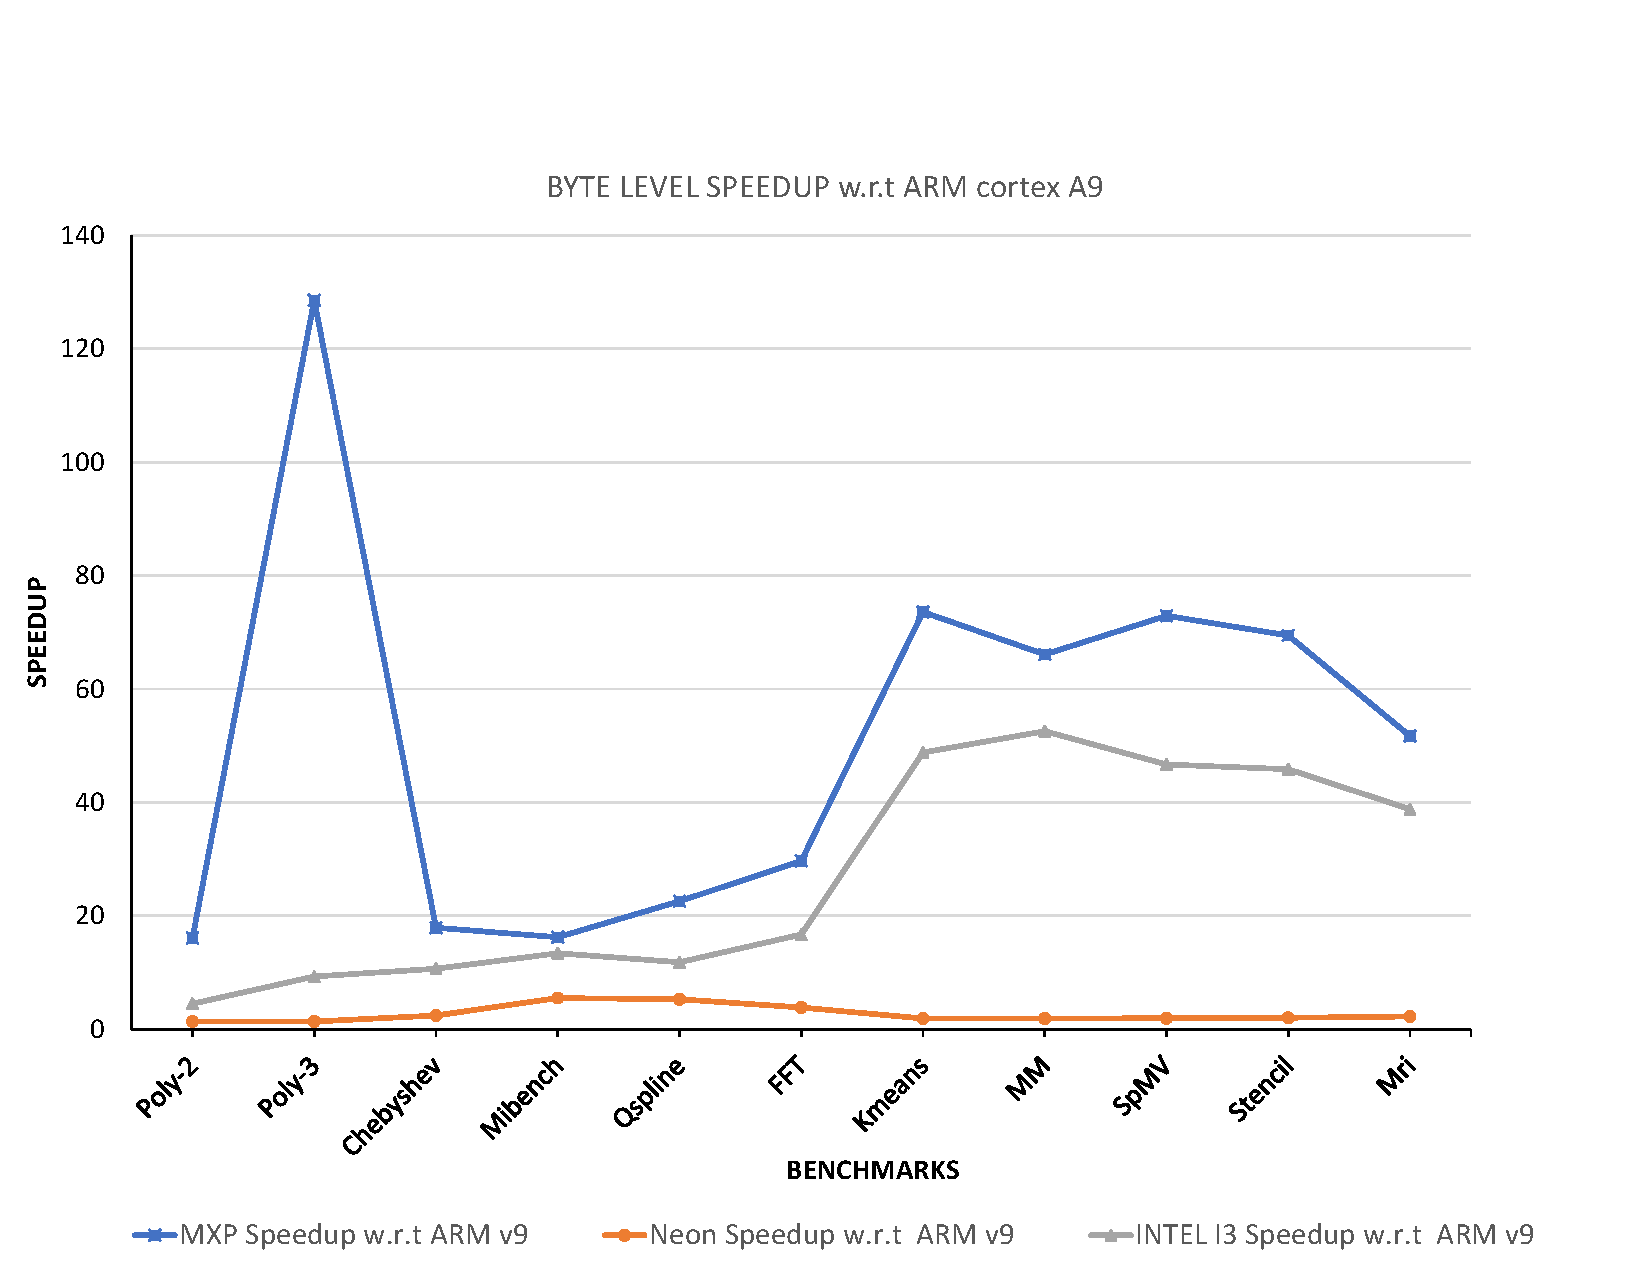
\includegraphics[width=.7\textwidth]{images/speedupbyte.pdf}
%    	\caption{Byte(8-bits) level Speedup w.r.t ARM A9}
%    	\label{random:1000}
%    \end{figure}
%  
% 
%    
%    \begin{figure}
%    	\centering
%    	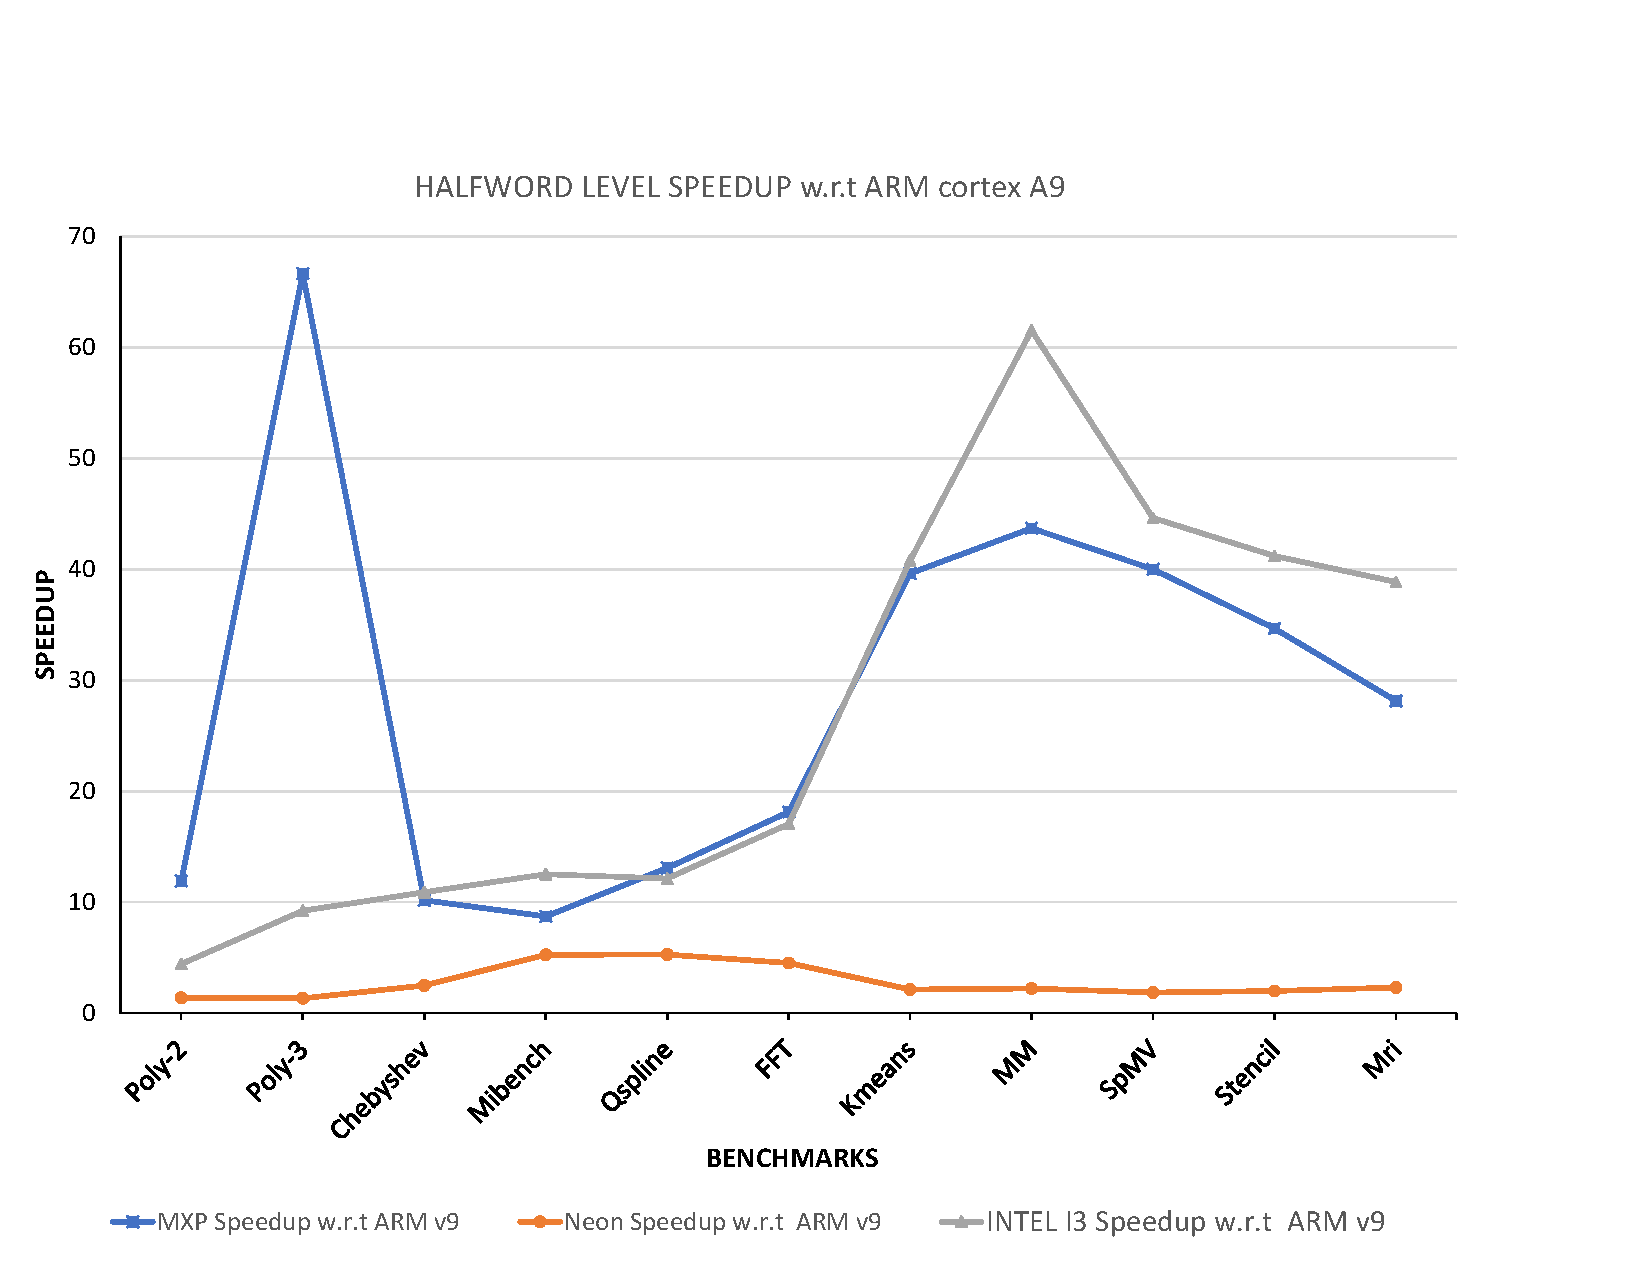
\includegraphics[width=.7\textwidth]{images/speeduphalf.pdf}
%    	\caption{Halfword(16-bits) level Speedup w.r.t ARM A9}
%    	\label{randomm:10000}
%    \end{figure}
%
%
%\begin{figure}
%	\centering
%	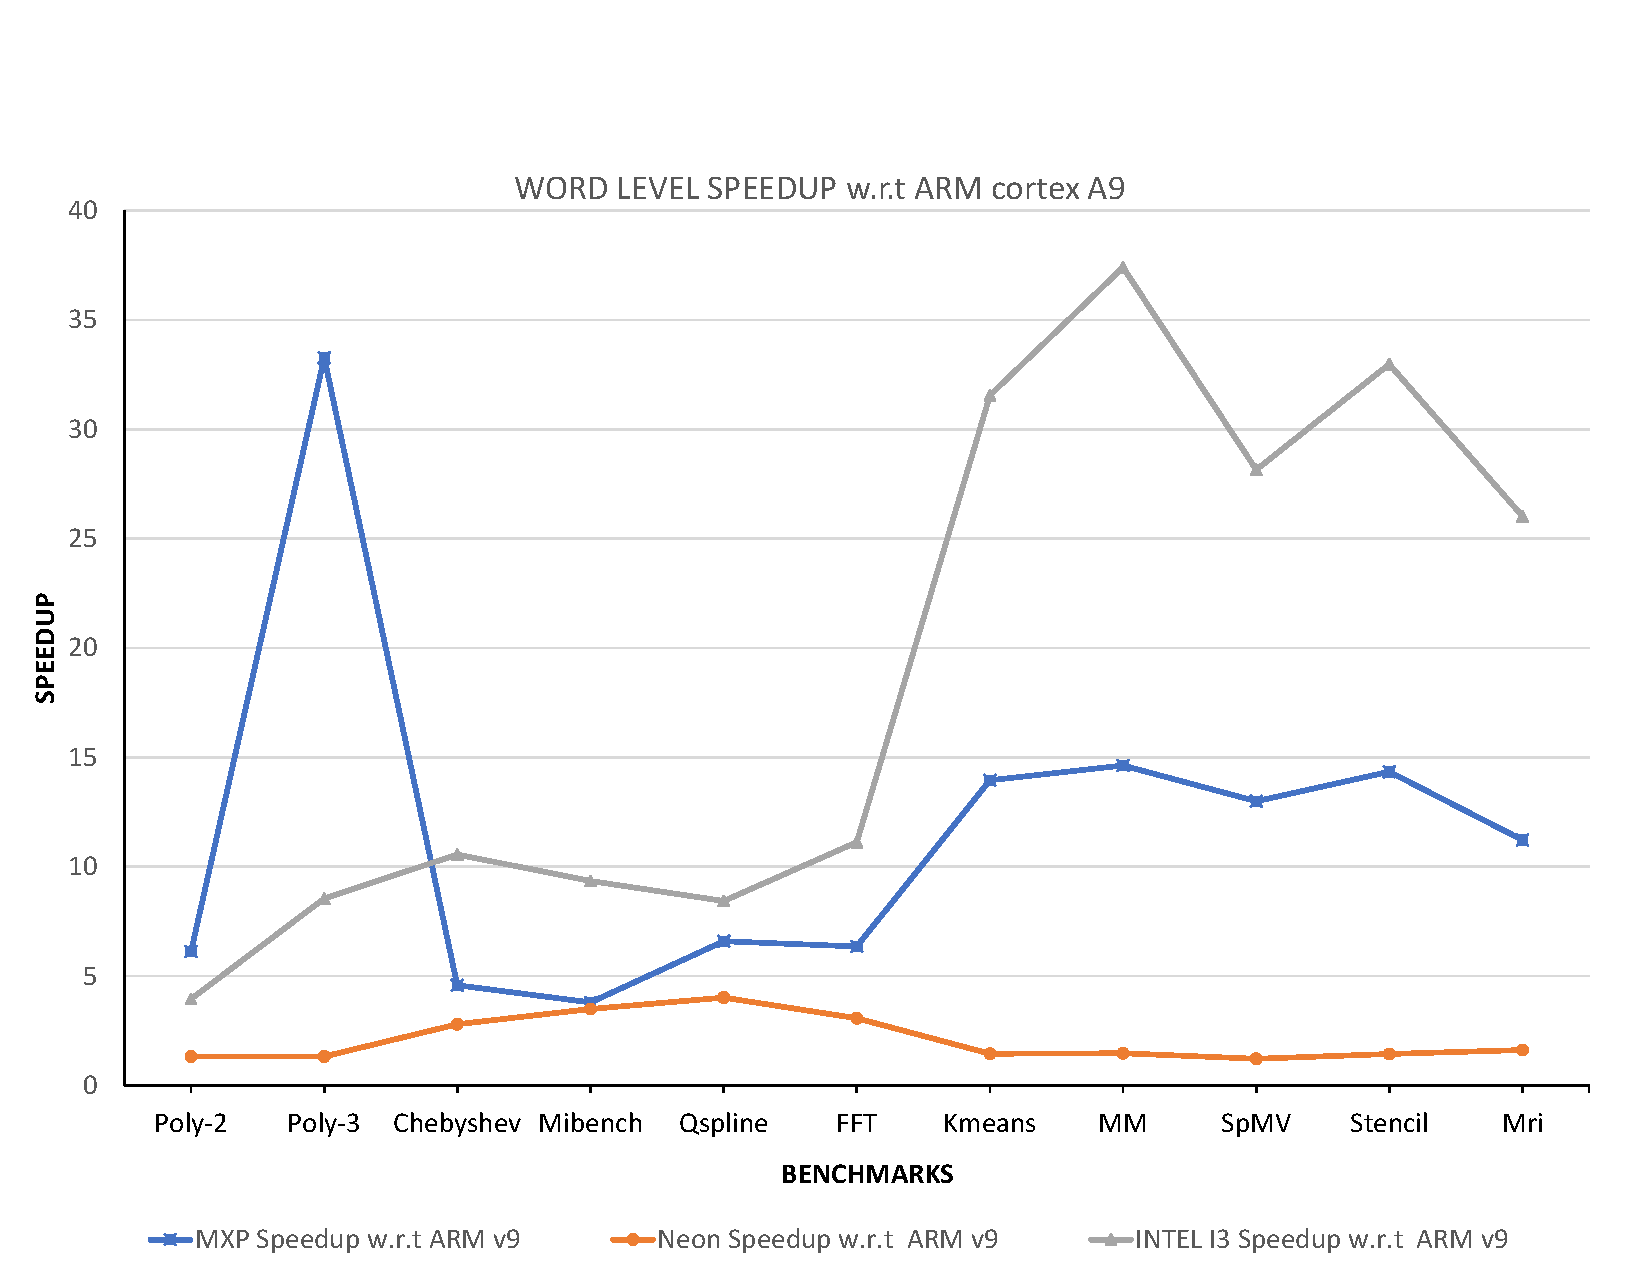
\includegraphics[width=.7\textwidth]{images/speedupword.pdf}
%	\caption{Word(32-bits) level Speedup w.r.t ARM A9}
%	\label{randommm:100000}
%\end{figure}
    
%    \section{Source Code for Measuring Performance}
    
%    The code for calculating the throughput for standard  kernels can be found in the below link:
    
%    Github Link : \url{https://github.com/AdhikariSaurabh/mxpbenchmarks}

%test
%
%\begin{figure}
%	\centering
%	\begin{tikzpicture}
%	\begin{axis}[
%	width  = 0.8*\textwidth,
%	height = 8cm,
%	%	major x tick style = transparent,
%	x tick label style={rotate=90, anchor=east, align=right,text width=2cm},
%	bar width=3pt,
%	ymajorgrids = true,
%	ylabel = {Throughput in $Gops/sec$},
%	symbolic x coords={poly2,poly3,chebyshev,mibench,qspline,fft,kmeans,mm,spmv,stencil,mri},
%	xtick = data,
%	nodes near coords,
%	ybar,
%	every node near coord/.append style={rotate=90, anchor=west,font=\scriptsize},
%	scaled y ticks = false,
%	enlarge y limits={upper,value=0.2},
%	%test
%	%	enlarge x limits=0.25,
%	ybar=2*\pgflinewidth,
%	legend cell align=left,
%	legend style={
%		at={(.5,-0.3)},
%		anchor=north,
%		legend columns=-1
%		column sep=0.5ex
%	}
%	]
%	\addplot[draw=black,fill=blue]
%	coordinates {(poly2, 0.1587) (poly3,0.2079) (chebyshev,0.142) (mibench,0.1279) (qspline,0.134) (fft,0.138) (kmeans,0.1279) (mm,0.134) (spmv,0.138) (stencil,0.134) (mri,0.138) };
%	
%	%	\addplot[draw=black,fill=orange]
%	%	coordinates  {(FFT, 0.278) (KMEANS,0.4702) (MM,0.3628) (SPMV,0.277) (STENCIL,0.308) (MRI,0.3201)};
%	
%	%	\addplot[draw=black,fill=yellow]
%	%	coordinates  {(FFT, 0.025) (KMEANS,0.0149) (MM,0.0097) (SPMV,0.00984) (STENCIL,0.00934) (MRI,0.0123)};
%	
%	%	\addplot[draw=black,fill=red]
%	%	coordinates {(FFT, 0.0769) (KMEANS,0.0216) (MM,0.01435) (SPMV,0.012) (STENCIL,0.0134) (MRI,0.02)};
%	\end{axis}	
%	\end{tikzpicture}
%	\caption{Comparing speedup in different benchmarks.}
%	\label{speedupcomparison}
%\end{figure}
%

